\documentclass[12pt, twoside]{article}
\usepackage{jmlda}
\newcommand{\hdir}{.}
\begin{document}

\title
    {Сходимость алгоритма аддитивной регуляризации тематических моделей}
\author
    { К.\,В.~Воронцов, И.\,А.~Ирхин}
    [К.\,В.~Воронцов$^{1}$, И.\,А.~Ирхин$^1$,]
\email
{vokov@forecsys.ru, ilirhin@gmail.com}
\organization
    {$^1$Московский Физико-Технический Институт, Россия, 141700, г. Долгопрудный, Институтский переулок, д. 9}
\abstract
{
Вероятностное тематическое моделирование применятся для выявления  латентных тем в больших коллекциях текстов. В каждом конкретном приложении тематическая модель должна удовлетворять примерно десятку различных требований одновременно. Поэтому, чтобы упростить процесс моделирования, Константином Воронцовым в 2014 году был предложен небайесовский многокритериальный подход, называемый Аддитивной Регуляризацией Тематических Моделей. Он основан на одновременной максимизации правдоподобия модели и множества дополнительных критериев-регуляризаторов. Преимущество АРТМ в том, что алгоритм выведен и реализован один раз в самом общем виде. На практике это позволяет строить сложные композитные модели с заданными свойствами.

Однако, до сих пор оставался открытым вопрос, при каких условиях этот алгоритм сходится. В данной работе такие условия были получены. Это было сделано за счёт интерпретации алгоритма АРТМ как GEM алгоритма. Неформально, алгоритм ARTM сходится, если регуляризатор воздействует на модель не слишком сильно, и есть определённая закономерность в обнулении и уменьшении основных параметров модели~--- условных вероятностей тем в документах и в слов в темах. Был проведён эксперимент, который подтвердил выполнение предложенных условий сходимости на практике.

 Кроме того, были предложены две модификации М-шага, которые немного улучшают сходимость без увеличения вычислительной сложности. 	
\bigskip

\noindent
\textbf{Ключевые слова}: \emph { компьютерный анализ текстов; тематическое моделирование; вероятностный латентный семантический анализ; EM алгоритм; латентное размещение Дирихле; аддитивная регуляризация; Байесовская регуляризация; сходимость; ARTM}
}

\titleEng
{Convergence of the algorithm of Additive Regularization of Topic Models}
\authorEng
    {K.\,V.~Vorontsov, I.\,A.~Irkhin}
    [ K.\,V.~Vorontsov$^{1}$, I.\,A.~Irkhin$^{1}$]
\organizationEng
    {$^1$Moscow Institute of Physics and Technology, 9 Institutskii per., Dolgoprudny, Moscow Region, 141700, Russia}
\abstractEng
    {
	\noindent
	\textbf{Background}: Probabilistic topic modeling is applied to identify latent topics in large collections of texts. Depending on each specific application the topic model must meet about ten different requirements simultaneously. So, to simplify the process of modeling, Konstantin Vorontsov proposed a non-Bayesian multi-criteria approach, called Additive Regularization of Topic Models(ARTM). It is based on the simultaneous maximization  of likelihood and a set of additional regularization criteria. The advantage of ARTM  is that its regularized Expectation Maximization algorithm is obtained and implemented once in the most general form. In practice, it gives an opportunity to build complex composite models with the desired properties. However, there was an open question about convergence test for ARTM algorithm.
	
	\noindent
	\textbf{Methods}: We interpreted the ARTM algorithm as GEM algorithm. It gave an opportunity to transfer results about convergence of GEM algorithms to the observed. Also it helped to find possible improvements of the algorithm.
	
	\noindent
	\textbf{Results}: We obtained the conditions of the convergence. Informally, ARTM algorithm converges if regularizer's effect on the model is not too big, and if there is a certain consistency in setting to zero and decreasing  of the main model parameters.  We conducted an experiment which confirmed that these conditions are satisfied in practice. In addition, we proposed two modifications of the M-step, which slightly improve the convergence without increasing the computational complexity.
	
	\noindent
	\textbf{Concluding Remarks}: We conducted an experiment which confirmed that the proposed conditions are satisfied in practice. In addition, the analysis of the ARTM algorithm lead us to two modifications of the M-step, which improve the convergence without increasing the computational complexity.
		
	\noindent
    	\textbf{Keywords}:  { text analysis; topic modeling; probabilistic latent semantic analysis; EM-algorithm; latent Dirichlet
allocation; additive regularization; Bayesian regularization; convergence; ARTM}
}

%данные поля заполняются редакцией журнала
\doi{10.21469/22233792}
\receivedRus{12.05.2016}
\receivedEng{May 12, 2016}

\maketitle
\linenumbers

\newcommand{\norm}{\mathop{\mathsf{norm}}\limits}

\section{Введение}
Тематическое моделирование~---это приложение машинного обучения к области анализа текстов. Тематическая модель коллекции текстовых документов относит каждый документ к некоторым темам и определеляет из каких слов (терминов) каждая тема состоит.

В вероятностной тематической модели каждая тема описывается дискретным распределением на множестве терминов,  а каждый документ~--- дискретным распределением на множестве тем. Делается предположение о том, что коллекция документов явдяется последовательностью терминов, которые выбираются случайно и независимо из смеси таких распределений, а затем ставится задача восстановить компоненты смеси по выборке.

Для  задачи вероятностного тематического моделирования  классическим решением является Вероятностный Латентный Семантический Анализ (Probabilistic Latent Semantic Analysis, PLSA). Эта модель  была предложена Томасом Хофманном в 1999 году \cite{hofmann1999probabilistic}. Основным её недостатком является то, что она задаёт закон порождения слов в документах, но не закон порождения самих документов \cite{daud2010knowledge}. Также  неясно, как оценивать слова, ранее не встречавшиеся в коллекции. Поэтому в 2003 году была предложена модель Латентного Размещения Дирихле (Latent Dirichlet Allocation, LDA) \cite{blei2003latent}, частично решающая эти проблемы. В LDA так же предполагается, что каждое слово в документе порождено некоторой латентной темой, однако, при этом в явном виде моделируется распределение слов в каждой теме, а также априорное
распределение тем в документе. С тех пор было предложено множество моделей, базирующихся на подходе LDA, которые постепенно усложняли вероятностную модель за счёт учёта связей между документами \cite{cohn2001missing,mccallum2005author,nallapati2008link}, метаданных о документах \cite{steyvers2004probabilistic} и информации о порядке слов в документе \cite{gruber2007hidden,wallach2006topic}.

Все эти модели объединяет общая схема. Сначала вводится вероятностная модель коллекции документов, а затем оценивается  апостериорное распределение  параметров. Для этого существует набор основных алгоритмов. Ниже приводится их краткий обзор.

EM алгоритм (Expectation Maximization) \cite{bilmes1998gentle} обычно используется для  точного оценивания параметров. Например, он используется для решения задачи PLSA. Основными недостатками метода являются быстрый рост количества параметров от числа слов, тем и документов, а также тот факт, что у функции правдоподобия большое число локальных максимумов, как следствие, алгоритм сильно зависит от начального приближения. Стоит отметить, что точное оценивание апостериорных распределений может требовать больших вычислительных затрат. В этом случае обычно используются вариационные методы \cite{jordan1999introduction}, являющиеся частным случаем EM алгоритма. Они  позволяют оценивать нижние и верхние доверительные границы для значений скрытых переменных в наблюдаемом документе. Однако, эти методы обладают теми же недостатками, что и исходный ЕМ алгортим.

Методы Монте-Карло для марковских цепей (Markov chain Monte Carlo, MCMC) \cite{gilks1996introducing,andrieu2003introduction} широко примяняются как эффективные методы приближенной процедуры сэмплирования значений из распределений высоких размерностей. Наиболее часто используется сэмплирование Гиббса \cite{griffiths2004finding}.  Обычно оно применяется, если слишком затрано вычислять и хранить функции распределения,  но не генерировать случайные выборки из этого распределения. В этом случае исходное распределение заменяется эмпирической оценкой, полученной по  сэмплированной из него выборке. Основным недостатком таких методов является время их работы: чтобы получить хорошее приближение распределения, требуется сэмплировать много объектов, что может быть очень трудоёмко. 

Также эти методы объединяет следующая проблема:  для каждой конкретной задачи требуется перестраивать вероятностную модель и заново строить байесовский вывод. Чтобы обойти обозначенные недостатки описанных алгоритмов, и в итоге получить простую, но гибкую и легко расширяемую модель для вероятностного тематического моделирования, был предложен подход Аддитивной Регуляризации Тематических Моделей (Additive Regularization for Topic Models, ARTM) \cite{vorontsov2014additive,vorontsov2014tutorial,vorontsov2015additive}. Это многокритериальный подход, в котором к основному критерию добавляется взвешенная сумма регуляризаторов. За счёт аддитивности алгоритм ARTM  выведен и реализован один раз в самом общем виде, и поэтому оптимизация любых моделей  производится при помощи одного и того же итерационного процесса. Гибкость подхода заключается в том, что, чтобы добавить новый регуляризатор, нужно лишь знать его частные производные по параметрам модели. За счёт вышесказанного можно утверждать, что ARTM~---  это не очередная тематическая модель, а общий подход к их  построению и комбинированию. 

Однако, открытым остаётся вопрос о сходимости предложенного в рамках ARTM алгоритма. Известно, что на практике алгоритм сходится, тем не менее, теоретического обоснования алгоритма не было предложено. Итерации алгоритма ARTM можно проинтерпретировать как итерации Generalized Expectation Maximization (GEM) алгоритма \cite{dempster1977maximum} в случае наличия априорного распределения. Условия сходимости GEM алгоритмов хорошо изучены \cite{wu1983convergence}, их можно перенести их на алгоритм ARTM и получить ограничения на регуляризаторы, а также понять, как стоит изменить алгоритм, чтобы улучшить его сходимость.


\section{Аддитивная регуляризация тематических моделей}
В главе будут введены используемые в работе обозначения и описаны алгоритмы PLSA и ARTM.
\paragraph{Постановка задачи и обозначения}
\label{subsec:denotes}
Пусть $D$~--- множество (коллекция) текстовых документов, $W$~--- множество (словарь) всех употребляемых в них терминов (слов или словосочетаний). Каждый документ $d \in D$ представляет собой последовательность $n_d$ терминов $(w_1, . . . , w_{n_d})$ из словаря $W$. Термин может повторяться в документе много раз. Пусть существует конечное множество тем $T$, и каждое употребление термина $w$ в каждом документе $d$ связано с некоторой темой $t \in T$, которая не известна. Формально, тема определяется как дискретное (мультиномиальное) вероятностное распределение в пространстве слов заданного словаря $W$.

Введем дискретное вероятностное пространство $D \times W \times T$. Тогда коллекция документов может быть рассмотрена как множество троек $(d, w, t)$, выбранных случайно и независимо из дискретного распределения $p(d, w, t)$. При этом документы $d \in D$ и термины $w \in W$ являются наблюдаемыми переменными, тема $t \in T$ является латентной (скрытой) переменной.

Требуется найти распределения терминов в темах $p(w \cond t) \equiv \phi_{wt}$ для всех тем $t \in T$ и распределения тем в документах $p(t \cond d) \equiv \theta_{td}$ для всех документов $d \in D$. При этом делается ряд допущений.

Принимается гипотеза условной независимости $p(w \cond d,t) = p(w \cond t)$, и  по формуле полной вероятности получается вероятностная модель порождения документа $d$:
\[
p(w \cond d) = \sum_{t \in T} p(w \cond d,t)p(t \cond d) = \sum_{t \in T}p(w \cond t)p(t \cond d)=\sum_{t \in T}\phi_{wt}\theta_{td}
\]

Введем следующие обозначения:

$p_{tdw} \equiv p(t \cond d,w)$~--- вероятность того, что появление термина $w$ в документе $d$ связано с темой $t$;

$n_{dwt}$~--- число троек $(d,w,t)$ во всей коллекции. Другими словами, это число появлений термина w в связи с темой t в документе d;

$n_{dw} = \sum_{t \in T} n_{dwt}$~--- число вхождений термина w в документ $d$,  наблюдаемая величина;

$n_{td} = \sum_{w \in d} n_{dwt}$~--- число вхождений  терминов, связанных с темой t в документ $d$;

$n_{wt} = \sum_{d \in D} n_{dwt}$~--- число появлений термина w в связи с темой $t$ во всех документах коллеккции $D$;

$n_{w} = \sum_{d \in D} n_{dw}$~--- число вхожений термина w в коллекцию;

$n_{d} = \sum_{t \in T} n_{td}$~--- длина документа $d$;

$n_{t} = \sum_{w \in W} n_{wt}$~--- <<длина темы>> \ \ $t$, то есть число появления  в коллекции терминов, связанных с темой $t$;

$n = \sum_{d \in D}\sum_{w \in d}\sum_{t \in T} n_{dwt}$~--- длина коллекции.

\noindentПравдоподобие~---  это плотность распределения выборки $D$:
\[
p(D)=\prod^n_{i=1}p_i(d,w)=\prod_{d \in D}\prod_{w \in d}p(d,w)^{n_{dw}}
\]

\noindentРассмотрим вероятностную тематическую модель $p(D,\Phi,\Theta)$, где 

$\Phi=(\phi_{wt})_{W \times T}$~--- искомая матрица терминов тем, $\phi_{wt} \equiv p(w \cond t)$,

$\Theta=(\theta_{td})_{T \times D}$~--- искомая матрица тем документов, $\theta_{td}\equiv p(t \cond d)$.

\noindentЗапишем задачу максимизации правдоподобия:
\[
p(D,\Phi,\Theta)=C\prod_{d \in D}\prod_{w \in d}p(d,w)^{n_{dw}}=\prod_{d \in D}\prod_{w \in d}p(d \cond w)^{n_{dw}}Cp(d)^{n_{dw}} \to \max_{\Phi,\Theta},
\]
где $C$~--- нормировочный множитель, зависящий только от чисел $n_{dw}$. Прологарифмируем правдоподобие, получив задачу максимизации:
\begin{equation}
\label{plsa_optimization}
L(D,\Phi,\Theta)=\sum_{d \in D}\sum_{w \in d}n_{dw}\ln\sum_{t \in T}\phi_{wt}\theta_{td} \to \max_{\Phi,\Theta}
\end{equation}
при ограничениях неотрицательности и нормировки
\[
\left\{
	\begin{aligned}
		\phi_{wt} \geq 0,~~\theta_{td} \geq 0\\
		\sum_{w \in W} \phi_{wt} = 1,~~\sum_{t \in T} \theta_{td}  = 1.
	\end{aligned}
\right.
\]
\paragraph{Итоговый алгоритм}

Описанная оптимизационная задача решается при помощи ЕМ алгоритма \cite{hofmann1999probabilistic}:

\noindent\textbf{E-шаг}

На E-шаге, используя текущие значения параметров $\phi_{wt}$ и $\theta_{td}$, по формуле Байеса вычисляются значения условных вероятностей:

$p_{tdw} \equiv p(t \cond d,w) = \frac {p(w \cond t)p(t \cond d)} {p(w \cond d)} = \frac {\varphi_{wt}\theta_{td}} {\sum_s\varphi_{ws}\theta_{sd}}$.

\noindent\textbf{М-шаг}

На M-шаге решается обратная задача: по условным вероятностям тем $p_{tdw}$ вычисляются новые приближения $\phi_{wt}$ и $\theta_{td}$.
Можно заметить, что величина $n_{dwt}=n_{dw}p(t \cond d,w)=n_{dw}p_{tdw}$ оценивает число вхождений термина $w$ в документ $d$, связанных с темой $t$. При этом оценка не всегда является целым числом. Просуммировав $n_{dwt}$ по документам $d$ и по терминам $w$, получим оценки:

$n_{wt}=\sum_{d \in D} n_{dwt}$,~~$n_t = \sum_{w \in W}n_{wt}$

$n_{td}=\sum_{w \in d} n_{dwt}$,~~$n_d = \sum_{t \in T}n_{td}$

$\phi_{wt}=\frac{n_{wt}}{n_t}$,~~$\theta_{td} = \frac{n_{dt}}{n_{d}}$


\paragraph{Добавление регуляризатора}

На оптимизационную задачу накладываются дополнительные ограничения. Подход ARTM \cite{vorontsov2014additive,vorontsov2014tutorial,vorontsov2015additive} основан на идее многокритериальной регуляризации. Он позволяет строить модели, удовлетворяющие многим ограничениям одновременно. Каждое ограничение формализуется в виде регуляризатора~--- оптимизационного критерия $R_i(\Phi,\Theta)\to\max$, зависящего от параметров модели. Взвешенная сума всех таких критериев $R(\Phi,\Theta) = \sum_{i=1}^k \tau_i R_i(\Phi,\Theta)$ максимизируется совместно с основным критерием правдоподобия.

\begin{equation}
\label{artm_optimization}
\sum_{d\in D} \sum_{w\in d} n_{dw}\log \sum_{t\in T} \phi_{wt}\theta_{td} \;+\; R(\Phi,\Theta)\;\to\; \max_{\Phi,\Theta},
\end{equation}
при тех же ограничениях нормировки и неотрицательности.

Применение теоремы Каруша-Куна-Таккера позволяет получить систему уравнений для стационарных точек данной оптимизационной задачи. Решение системы методом простых итераций даёт EM алгоритм со следующими формулами M-шага:
\[
\left\{
	\begin{aligned}
\phi_{wt} = \norm_w  \left(n_{wt} + \phi_{wt}\frac{\partial R}{\partial\phi_{wt}}\right),\\
\theta_{td} = \norm_t  \left(n_{td} + \theta_{td}\frac{\partial R}{\partial\theta_{td}}\right),
	\end{aligned}
\right.
\]
где $\norm_x(y) = \frac{\max(y, 0)}{\sum\limits_x \max(y, 0)}$. Операция $\max(y, 0)$ называется положительной срезкой.

Приведём примеры наиболее часто используемых регуляризаторов. Более подробное описание есть в статьях \cite{vorontsov2014additive, vorontsov2014tutorial, vorontsov2015additive}:
\begin{enumerate*}
\item $R = \alpha \sum\limits_{w, t} \ln \phi_{wt}$~--- регуляризатор сглаживания.
\item $R = -\alpha \sum\limits_{w, t} \ln \phi_{wt}$~--- регуляризатор разреживания.
\item $R = -\sum\limits_{w \neq u, t} \phi_{wt} \phi_{ut}$~--- регуляризатор декоррелирования.
\item $R = \sum\limits_{w \neq u, t} C_{uw}\left( \phi_{wt}  - \phi_{ut} \right)^2$~--- регуляризатор когерентности.
\item $R = \sum\limits_{s \neq t, d} C_{st}\left( \theta_{td}  - \theta_{sd} \right)^2$~--- регуляризатор связей документов.
\end{enumerate*}

\section{Сходимость алгоритма ARTM}

В главе будут изложены основные теоретические результаты работы. Будут доказаны теоремы о сходимости алгоритма ARTM, используя результаты о сходимостях GEM алгоритмов. Также будет проведена оценка изменения функционалов на М-шаге алгоритма ARTM, и будут предложены возможные модификации для формулы М-шага, улучшающие оптимизацию. 
	
\paragraph{ARTM как GEM алгоритм}
\label{subsec:artmasgem}

В ARTM ставится задача максимизации следующего функционала:
\[
L + R = \sum_{w,d} n_{dw} \ln\sum_t \phi_{wt} \theta_{td} +  R(\Phi, \Theta) \to \max.
\]
Вводится дополнительный функционал:
\[
	Q(\Phi, \Theta, \Phi', \Theta') = \sum\limits_{d, w, t} n_{dw} p'_{tdw} \ln{\phi_{wt}\theta_{td}} + R(\Phi, \Theta),
\]
где за $p'_{tdw}$ обозначено $\frac{\phi'_{wt} \theta'_{td}}{\sum\limits_t \phi'_{wt} \theta'_{td}}$.\\

Согласно требованию GEM алгоритма требуется увеличивать значение данного функционала по $\Phi$ и $\Theta$ в сравнении с $Q(\Phi', \Theta', \Phi', \Theta')$ на каждой итерации. Запишем задачу максимизации $Q$:
\[
Q(\Phi, \Theta, \Phi', \Theta') \to \max_{\Phi, \Theta}.
\]

Применив теорему Куна-Таккера,  получим, что стационарная точка $Q$ должна удовлетворять следующей системе:
\[
\left\{
	\begin{aligned}
		\phi_{wt}= \norm_w \left( \sum\limits_d n_{dw} p'_{tdw} + \phi_{wt} \frac{\partial{R}}{\partial{\phi_{wt}}} \right),\\
		\theta_{td} = \norm_t \left( \sum\limits_w n_{dw} p'_{tdw} + \theta_{td} \frac{\partial{R}}{\partial{\theta_{td}}} \right).
	\end{aligned}
\right.
\]

В итоге получаем систему уравнений, похожих на итерации ARTM. Это означает, что каждую итерацию ARTM можно интерпретировать как попытку приблизить решение максимизационной задачи функционала $Q$, итерируя систему уравнений для стационарной точки $Q$. В зависимости от того, какая точка будет браться начальной при итерировании системы уравнений, получаются разные варианты алгоритма ARTM.

Если начальное приближение~--- это $(\phi_{wt}, \theta_{td})$, то получаем итерации:
\begin{equation}
\label{artm_original}
\left\{
	\begin{aligned}
		\phi_{wt} = \norm_w \bigg( n_{wt} + \tau\phi_{wt} \frac{\partial{R}}{\partial{\phi_{wt}}} \left( \phi_{wt}, \theta_{td}\right) \bigg),\\
		\theta_{td} = \norm_t \bigg( n_{td} + \tau\theta_{td} \frac{\partial{R}}{\partial{\theta_{td}}} \left( \phi_{wt}, \theta_{td}\right) \bigg).
	\end{aligned}
\right.
\end{equation}
Эту формулу будем в дальнейшем называть стандартной формулой М-шага. Если же считать, что начальное приближение~---  это $\left(\frac{n_{wt}}{n_t}, \frac{n_{td}}{n_d}\right)$, то:
\begin{equation}
\label{artm_unbiased}
\left\{
	\begin{aligned}
		\phi_{wt}= \norm_w \bigg( n_{wt} + \tau \frac{n_{wt}}{n_t} \frac{\partial{R}}{\partial{\phi_{wt}}} \left(\frac{n_{wt}}{n_t}, \frac{n_{td}}{n_d}\right) \bigg),\\
		\theta_{td} = \norm_t \bigg(n_{td} + \tau \frac{n_{td}}{n_d} \frac{\partial{R}}{\partial{\theta_{td}}} \left(\frac{n_{wt}}{n_t}, \frac{n_{td}}{n_d}\right) \bigg).
	\end{aligned}
\right.
\end{equation}
Эту формулу будем называть несмещённой модификацией М-шага.

Таким образом, интерпретируя ARTM как итерации GEM алгоритма, можно использовать результаты о сходимости GEM алгоритма.

\paragraph{Итерации ARTM в обобщённом виде}
Итерации ARTM можно записать в следующем виде: 

\textbf{E-step:}   
 
\begin{equation}
\label{artm_generalE}
\begin{aligned}
\qquad& p_{tdw} = \norm_t \phi_{wt} \theta_{td}.
\end{aligned}
\end{equation}

\textbf{M-step:}
\begin{equation}
\label{artm_generalM}
\begin{aligned}
\qquad& n_{wt} = \sum\nolimits_{d} n_{dw} p_{tdw},~~n_{td} = \sum\nolimits_{w} n_{dw} p_{tdw},\\    
\qquad& r_{wt} =  \phi_{wt}\frac{\partial R}{\partial\phi_{wt}},~~ r_{td} =  \theta_{td}\frac{\partial R}{\partial\theta_{td}},\\
\qquad& \phi_{wt}  = \norm_w \left(n_{wt} + r_{wt} \right),~~\theta_{td} = \norm_t  \left(n_{td} + r_{td}\right).\\
\end{aligned}
\end{equation}
Величины $r_{wt}$ и $r_{td}$ будем называть регуляризационными добавками. Они являются функциями от $\Phi$ и $\Theta$. Фактичеки, именно от их свойств зависит всё поведение алгоритма.


\paragraph{Теорема о сходимости}
 В работе Wu \cite{wu1983convergence} были сформулированы достаточные условия для сходимости GEM алгоритма. Чтобы их сформулировать, нужно сначала ввести одно определение.
\begin{Definition}
Будем говорить, что $A\colon X \to 2^X$~--- замкнутое point-to-set отображение, если из $x_k \to x$, $x \in X$, $y_k \to y$ и $y_k \in A(x_k)$ следует, что $y \in A(x)$.
\end{Definition}

Cформулируем теорему из работы Wu, изменив обозначения под ARTM:
\begin{Theorem} \label{Theorem_wu} 
Пусть $\{(\Phi^k, \Theta^k)\}$~--- траектория итерационного процесса, сгенерированная правилом $(\Phi^{k+1}, \Theta^{k+1}) \in M((\Phi^k, \Theta^k))$, где $M$~--- закмнутое point-to-set отображение. Пусть также значение $L +  R$ конечно и не уменьшается на итерациях алгоритма, но при этом ограничено сверху, $|| \phi^k_{wt} - \phi^{k+1}_{wt}|| \to 0$ и $|| \theta^k_{td} - \theta^{k+1}_{td}||\to 0$, а множество стационарных точек $L +  R$ дискретно. Тогда $(\Phi^k, \Theta^k)$ сходится к некоторой стационарной точке $L +  R$.
\end{Theorem}

Сходимость ARTM будет сведена к этой теореме, но для этого потребуется ввести новые определения.

\begin{Definition}
\label{strongreg}
Будем говорить, что регуляризатор $ R$ обладает свойством $\delta$-регулярности, если на итерациях алгоритма ARTM $\forall t~\exists w \colon~n_{wt} + r_{wt} > \delta$ и $\forall d~\exists t \colon~n_{td} + r_{td} > \delta$. Если регуляризатор  обладает свойством $\delta$-регулярности при некотором $\delta > 0$, то будем говорить, что регуляризатор сильно регулярен, при $\delta=0$ будем говорить, что регуляризатор регулярен.
\end{Definition}

Регулярность позволяет утверждать, что итерации ARTM корректно определены. Сильная же регулярность позволяет утверждать, что преобразования, которые производятся на итерациях алгоритма, не только определены, но и непрерывны. Выполнение этого свойства на практике  можно гарантировать следующим образом: если значение $n_{wt} + r_{wt}$ становится меньше $\delta$, то вся тема зануляется  и выкидывается, таким образом происходит селекция тем. Зануления тем будут происходить, если  изначально задаётся заведомо большое число для их количества. Темы, содержащие слишком мало слов, удаляются, поскольку значение $n_t$ получается небольшим. Для оставшихся тем, условие сильной регулярности будет выполнено по построению.
 
\begin{Definition}
Будем говорить, что регуляризатор $R$ сохраняет 0, если на итерациях алгоритма ARTM $n_{wt} = 0 \Rightarrow \phi_{wt} = 0$ и $n_{td} = 0 \Rightarrow \theta_{td} = 0$.
\end{Definition}

Это определение формализует следующие свойство итераций: если на какой-либо итерации значение $\phi_{wt}$ стало равным нулю, то оно будет оставаться нулевым на последующих итерациях, и аналогично для $\theta_{td}$. Для регуляризатора свойство проверяется аналитически. На практике все регуляризаторы им обладают.

\begin{Definition}
\label{sparsereg}
Будем говорить, что регуляризатор $ R$ $\epsilon$-разреживающий, если на итерациях алгоритма ARTM $\phi_{wt}, \theta_{td} \notin (0, \epsilon)$.
\end{Definition}

Предложенное свойство позволяет формально учесть машинную точность (с этой точки зрения все регуляризаторы будут $\epsilon$-разреживающими). Однако с точки зрения практики есть одна интересная особенность. Регуляризатор разреживания используется, чтобы каждой теме принадлежало лишь небольшое число слов. Фактически,  $n_{wt}$ зануляется, если его значение меньше $\alpha$, таким образом, после нормировки выполнено $\phi_{wt} \geq \frac{n_{wt} - \alpha}{n_t} > 0$.  На реальных коллекциях очень часто происходит следующее: характерные слова темы $t$ имеют существенное значение $n_{wt}$ (например, больше 1), а нехарактерные постепенно зануляются. В итоге получаем, что, начиная с некоторой итерации, $\phi_{wt} \notin (0, \frac{1-\alpha}{n_t})$.

Есть альтернативный способ добиться описанного ограничения: достаточно заменить регуляризатор разреживания на $-\alpha \ln \min(\phi_{wt}, \alpha)$. В этом случае получим, что на М-шаге зануляются выражения меньше $\alpha$ и не изменяются остальные значения. В этом случае $\phi_{wt}\notin (0, \frac{\alpha}{n_t})$.

\begin{Definition}
\label{fairreg}
Будем говорить, что регуляризатор $R$ корректный, если на итерациях алгоритма ARTM $n_{dw} > 0 \Rightarrow \exists t\colon p_{tdw} > 0$.
\end{Definition}

Это свойство~--- чистая формальность. Если будут производиться разреживания, то необходимо случайно не занулить элемент матрицы $\Phi \Theta$ для которого $n_{dw} > 0$. Это привело бы к падению $L$ до -$\infty$.  Корректность требует, чтобы такого не происходило. На практике оно обычно будет выполнено за счёт фоновых тем\cite{vorontsov2014tutorial}, поскольку они, как правило, дают небольшие вероятности для всех слов.

\begin{Theorem} \label{Theorem_neighbour_zero1} Пусть $R$~--- дифференцируемая функция при $\phi_{wt}, \theta_{td} \in (0, 1]$, причем, как регуляризатор сохраняющая 0, корректная, $\epsilon$-разреживающая и обладающая свойством регулярности. Также допустим,  что значение $Q(\Phi, \Theta, \Phi', \Theta')$  и не уменьшается в сравнении с $Q(\Phi', \Theta', \Phi', \Theta')$, начиная с некоторой итерации. Тогда при $d$ и $w$ таких, что $n_{dw} > 0$ выполнено:
\[
KL(p_{tdw}^{k}||p_{tdw}^{k+1}) \to 0 \text{ при }  k \to \infty.
\]
\end{Theorem}
\begin{Proof}
Поскольку регуляризатор сохраняет 0, то с некоторой итерации множество позиций с нулевыми значениями в матрице $\Phi$ и $\Theta$ стабилизируется и не будет больше изменяться. Это очевидно следует из того факта, что  множество всех позиций конечно. Обозначим стабилизировавшееся множество ненулевых позиций матриц $\Phi$ и $\Theta$ за $\Omega$. В силу того, что регуляризатор $\epsilon$-разреживающий, значения $\Phi$ и $\Theta$ в позициях из $\Omega$ будут $\geq \epsilon$. Но $R$~--- дифференцируемая функция при $\phi_{wt}, \theta_{td} \in [\epsilon, 1]$, а, значит, непрерывная и ограниченная. В силу корректности регуляризатора $Q(\Phi, \Theta, \Phi', \Theta')$  будет иметь конечные значения.
Заметим, что $Q$ можно переписать следующим образом:
\[
Q(\Phi, \Theta, \Phi', \Theta') = L(\Phi, \Theta) +  R(\Phi, \Theta) + \sum\limits_{d, w, t} n_{dw} p'_{tdw} \ln{p_{tdw}}.
\]
Пусть на М-шаге был переход в точку $\Phi'', \Theta''$. Значения функционала $Q$ не уменьшаются, значит,
\[
	Q(\Phi'', \Theta'', \Phi', \Theta') \geq Q(\Phi', \Theta', \Phi', \Theta').
\]
Подставим вместо $Q$ его выражение:
\[
	L(\Phi'', \Theta'') + R(\Phi'', \Theta'') + \sum\limits_{d, w, t} n_{dw} p'_{tdw} \ln{p''_{tdw}}  \geq L(\Phi', \Theta') +  R(\Phi', \Theta') + \sum\limits_{d, w, t} n_{dw} p'_{tdw} \ln{p'_{tdw}}
\]
\[
	\Delta(L +  R) \geq  \sum\limits_{d, w, t} n_{dw} p'_{tdw} \ln{\frac{p'_{tdw}}{p''_{tdw}}} = \sum\limits_{d, w} n_{dw} KL(p'_{dw} || p''_{dw}) \geq 0.
\]
Таким образом, $L +  R$  тоже не уменьшается. Но это ограниченная функция, значит, $(L + R)^{k}$ сходится при $k \to \infty$. Более того, при $n_{dw} > 0$:
\[
	KL(p_{tdw}^{k}||p_{tdw}^{k+1}) \leq \Delta (L +  R)^{k} \to 0.
\]
\end{Proof}

\begin{Corollary}
\label{corolary_first}
Если в дополнение к условиям Теоремы \ref{Theorem_neighbour_zero1} $R$ сильно регулярен, а $r_{wt}$ и $r_{td}$ непрерывны, то:
\[
|\phi_{wt}^{k} - \phi_{wt}^{k+1}| \to 0 \text{ и } |\theta_{td}^{k} - \theta_{td}^{k+1}| \to 0
\]
\end{Corollary}
\begin{Proof}
По неравеству Пинскера \cite{topsoe2000some} $||A - B||_1 \leq 2\sqrt{KL(A||B)}$. Поэтому сходимость по $KL$ влечёт за собой сходимость по $l_1$ норме. Осталось заметить, что в потребованных условиях  $\phi_{wt}$ и $\theta_{td}$ являются непрерывными функциями от $p_{tdw}$. А значит, сходимость вторых влечёт за собой сходимость первых.
\end{Proof}
\begin{Corollary}
В условия Следствия 1 все предельные точки последовательности $(\Phi^k, \Theta^k)$ являются стационарными точками $L +  R$ при каком-то ограничении на множество нулевых позиций в матрицах $\Phi$ и $\Theta$.
\end{Corollary}
\begin{Proof}
Опишем коротко идею доказательства,  более подробно и формально оно описано в \cite{wu1983convergence}. Пусть  $\phi^0, \theta^0$~--- предельная точка последовательности $(\Phi^k, \Theta^k)$. Известно, что выполнено:
\[
Q(\Phi, \Theta, \Phi^0, \Theta^0) =  L(\Phi, \Theta) +  R(\Phi, \Theta) + \sum\limits_{d, w, t} n_{dw} p^0_{tdw} \ln{p_{tdw}}.
\]
Поскольку $\phi^0, \theta^0$ ~--- предельная точка, то значение $Q$ уже нельзя увеличить, не изменяя сложившееся множество ненулевых позиций, а, значит, производная по $\phi$ и по $\theta$ левой части равна нулю при соответсвующем ограничении. При $\phi = \phi^0$ и $\theta = \theta^0$ KL достигает минимума, а, значит, и его производные равны нулю. Таким образом получается, что и производные $L +  R$ равны нулю, что и требовалось доказать.
\end{Proof}
\begin{Corollary}
Если в дополнение к условиям Следствия \ref{corolary_first}, множество стационарных точек $L +  R$ дискретно при любом  ограничении на множество нулевых позиций в матрицах $\Phi$ и $\Theta$, то $\phi_{wt}^{k}$ и $\theta_{td}^{k}$ сходятся к стационарной точке $L +  R$ при некотором ограничении множества нулевых позиций.
\end{Corollary}
\begin{Proof}
Положим $M((\Phi, \Theta)) = \{artm(\Phi, \Theta)\}$, где под $artm(\Phi, \Theta)$ понимается применение формул \eqref{artm_generalE},\eqref{artm_generalM} к матрицам $\Phi$ и $\Theta$. В условиях Следствия 1 $artm$~--- непрерывное преобразование. Поэтому $M$~--- замкнутое point-to-set отображение. Остаётся заметить, что остальные условия Теоремы \ref{Theorem_wu} тоже выполнены.
\end{Proof}

Теперь можно описать, что происходит на итерациях алгоритма ARTM (в предположении увеличения $Q$). Итерации можно разбить на два этапа: селекция ненулевых позиций и оптимизация. На первом этапе при помощи регуляризатора выбирается множество ненулевых позиций итогового решения. Понятно, что параллельно ведётся и оптимизация $L + R$, но из-за наличия положительной срезки в нормировке на М-шаге этот этап очень сложно анализировать. Его стоит воспринимать как подготовка начального приближения. На втором этапе оптимизация выходит на первый план. В силу того, что множество нулевых позиций не изменяется, положительную срезку в формулах можно убрать. Это облегчает анализ, который будет проведён в соответсвующей главе.

\paragraph{Изменение регуляризированного правдоподобия на итерациях алгоритма ARTM}
Важным условием сходимости алгоритма ARTM является неуменьшение значения $Q$ на М-шаге.Далее изучается поведение алгоритма на М-шаге и проводятся оценки изменения функционалов $L$, $R$ и $Q$. На основании результатов анализа будет предложена  модификация М-шага (в дополнение к замене $\phi_{wt}$ и $\theta_{td}$ несмещёнными оценками).

Под $Q^{\prime}$ будем понимать $\sum\limits_{d, w, t} n_{dw} p'_{tdw} \ln{\phi_{wt}\theta_{td}}$. То есть $Q = Q^{\prime} +  R$.

Провести анализ суммарного изменения функционала $Q$ на М-шаге затруднительно. Поэтому предлагается разложить это преобразование на два этапа. Первый этап~--- максимизация $Q^{\prime}$:
\[
\left\{
	\begin{aligned}
		\phi_{wt} = \norm_w  n_{wt},\\
		\theta_{td} = \norm_t n_{td} .
	\end{aligned}
\right.
\]

Второй этап (назовём его регуляризационным преобразованием)~--- максимизация $R$:
\[
\left\{
\begin{aligned}
 \phi_{wt}  = \norm_w \left(n_{wt} + r_{wt} \right),\\
\theta_{td} = \norm_t  \left(n_{td} + r_{td}\right)
\end{aligned}
\right.
\]

Таким образом, изменения функционалов будут оцениваться  отдельно на каждом этапе. На первом происходит переход в точку $\left(\frac{n_{wt}}{n_t}, \frac{n_{td}}{n_d}\right)$, максимизируя $Q^{\prime}$, а на втором проводится максимизация $R$. 

Предлагается использовать следующую технику. Введём новую функцию $R^{\prime}$: $R^{\prime}(m_{wt}, m_{td}) = R\left( \frac{m_{wt}}{\sum\limits_w m_{wt}},  \frac{m_{td}}{\sum\limits_t m_{td}}\right) \equiv R\left( \frac{m_{wt}}{m_t},  \frac{m_{td}}{m_d}\right)$. Также введём обозначение $g_{wt} \equiv \frac{\partial{R^{\prime}}}{\partial{m_{wt}}}$ и $g_{td} \equiv \frac{\partial{R^{\prime}}}{\partial{m_{td}}}$. Обратим внимание, что это функции. Для них справедливо следующее утверждение:
\begin{State}
\label{Stategradientvalue}           
Для $g_{wt}$ и $g_{td}$ выполнено:
\begin{equation}
\label{rgradient}
\begin{aligned}
g_{wt} = \frac{1}{m_t} \sum_{u} \left(\frac{\partial{R}}{\partial{\phi_{wt}}}  -  \frac{\partial{R}}{\partial{\phi_{ut}}} \right)  \phi_{ut},\\
g_{td} = \frac{1}{m_d} \sum_{s} \left(\frac{\partial{R}}{\partial{\theta_{td}}}  -  \frac{\partial{R}}{\partial{\theta_{sd}}} \right)  \theta_{sd} .
\end{aligned}
\end{equation}
\end{State}
\begin{Proof}
$\phi_{wt} = \frac{m_{wt}}{\sum_w m_{wt}}$, поэтому
\[
\frac{\partial{\phi_{ut}}}{\partial{m_{wt}}} = \frac{\partial{ \frac{m_{ut}}{\sum\limits_v m_{vt}}}}{\partial{m_{wt}}} = \frac{ \frac{\partial{m_{ut}}}{\partial{m_{wt}}}}{\sum\limits_v m_{vt}} - \frac{m_{ut}}{(\sum\limits_v m_{vt})^2} = I\{u = w\} \frac{1}{m_t} - \frac{\phi_{ut}}{m_t} = \frac{1}{m_t}\left( 
 I\{u = w\} - \phi_{ut} \right).
\]
А, значит,
\[
\frac{\partial{R^{\prime}}}{\partial{m_{wt}}} = \sum_{u} \frac{\partial{R}}{\partial{\phi_{ut}}} \frac{\partial{\phi_{ut}}}{\partial{m_{wt}}} = \frac{1}{m_t} \left( \frac{\partial{R}}{\partial{\phi_{wt}}} - \sum_{u}  \frac{\partial{R}}{\partial{\phi_{ut}}} \phi_{wt} \right) = 
\]
\[
=\frac{1}{m_t} \left( \frac{\partial{R}}{\partial{\phi_{wt}}} - \sum_{u}  \frac{\partial{R}}{\partial{\phi_{ut}}} \phi_{ut} \right) = \frac{1}{m_t} \sum_{u} \left(\frac{\partial{R}}{\partial{\phi_{wt}}}  -  \frac{\partial{R}}{\partial{\phi_{ut}}} \right)  \phi_{ut}.
\]
Для $\frac{\partial{R^{\prime}}}{\partial{n_{td}}}$ формула доказывается аналогично.
\end{Proof}
\medskip

\noindentТеперь докажем следующую лемму:
\begin{Lemma}           
Для несмещённой модификации М-шага в ходе регуляризационного преобразования  без занулений угол  между вектором изменений и градиентом $R$ острый, если градиент ненулевой.
\end{Lemma}
\begin{Proof}
При регуляризационном преобразовании без занулений $\Delta n_{wt} =  \phi_{wt} \frac{\partial{R}}{\partial{\phi_{wt}}}$, а для несмещённой модификации $\phi_{wt} = \frac{n_{wt}}{\sum\limits_w n_{wt}}$. Отсюда
\[
\langle \Delta n, \nabla R^{\prime}(n_{wt}, n_{td})\rangle = \sum\limits_{w, t, u}  \frac{1}{n_{t}}  \left(  \frac{\partial{R}}{\partial{\phi_{wt}}}  -  \frac{\partial{R}}{\partial{\phi_{ut}}}  \right)  \frac{\partial{R}}{\partial{\phi_{wt}}} \phi_{wt} \phi_{ut}.
\]
Если переобозначить $u$ за $w$ и наоборот, то 
\[
\sum\limits_{w, t, u}  \frac{1}{n_{t}}  \left(  \frac{\partial{R}}{\partial{\phi_{wt}}}  -  \frac{\partial{R}}{\partial{\phi_{ut}}}  \right)  \frac{\partial{R}}{\partial{\phi_{wt}}} \phi_{wt} \phi_{ut}  = \sum\limits_{w, t, u}  \frac{1}{n_{t}}  \left(  \frac{\partial{R}}{\partial{\phi_{ut}}}  -  \frac{\partial{R}}{\partial{\phi_{wt}}}  \right)  \frac{\partial{R}}{\partial{\phi_{ut}}} \phi_{wt} \phi_{ut} = 
\]
\[
= \sum\limits_{w, t, u}  \frac{1}{n_{t}}  \left(  \frac{\partial{R}}{\partial{\phi_{wt}}}  -  \frac{\partial{R}}{\partial{\phi_{ut}}}  \right)  \left(-\frac{\partial{R}}{\partial{\phi_{ut}}}\right) \phi_{wt} \phi_{ut} = 
\]
\[
= \frac12 \left(\sum\limits_{w, t, u}  \frac{1}{n_{t}}  \left(  \frac{\partial{R}}{\partial{\phi_{wt}}}  -  \frac{\partial{R}}{\partial{\phi_{ut}}}  \right)  \frac{\partial{R}}{\partial{\phi_{wt}}} \phi_{wt} \phi_{ut} +  \sum\limits_{w, t, u}  \frac{1}{n_{t}}  \left(  \frac{\partial{R}}{\partial{\phi_{wt}}}  -  \frac{\partial{R}}{\partial{\phi_{ut}}}  \right)  \left(-\frac{\partial{R}}{\partial{\phi_{ut}}}\right) \phi_{wt} \phi_{ut} \right)= 
\]
\[
= \frac12 \sum\limits_{t, w, u}  \frac{1}{n_{t}} \left(  \frac{\partial{R}}{\partial{\phi_{wt}}}  -  \frac{\partial{R}}{\partial{\phi_{ut}}}  \right)^2 \phi_{wt} \phi_{ut} = \sum\limits_{t, w < u}  \frac{1}{n_{t}} \left(  \frac{\partial{R}}{\partial{\phi_{wt}}}  -  \frac{\partial{R}}{\partial{\phi_{ut}}}  \right)^2 \phi_{wt} \phi_{ut} \geq 0.
\]
Пусть достигается равенство, тогда $\frac{\partial{R}}{\partial{\phi_{wt}}}  =  \frac{\partial{R}}{\partial{\phi_{ut}}}$ для всех $u$ и $w$. Тогда
\[
\frac{\partial{R^{\prime}}}{\partial{n_{wt}}} = \frac{1}{n_t} \left( \frac{\partial{R}}{\partial{\phi_{wt}}} - \sum_{u}  \frac{\partial{R}}{\partial{\phi_{ut}}} \phi_{ut} \right) = \frac{1}{n_t} \left( \frac{\partial{R}}{\partial{\phi_{wt}}} - \sum_{u}  \frac{\partial{R}}{\partial{\phi_{wt}}} \phi_{ut} \right) =
\]
\[
=\frac{1}{n_t} \left( \frac{\partial{R}}{\partial{\phi_{wt}}} - \frac{\partial{R}}{\partial{\phi_{wt}}} \sum_{u} \phi_{ut} \right)  = \frac{1}{n_t} \left( \frac{\partial{R}}{\partial{\phi_{wt}}} - \frac{\partial{R}}{\partial{\phi_{wt}}} \right) = 0.
\]
Значит, градиент нулевой~--- противоречие. Поэтому, неравенство строгое и угол острый.
\end{Proof}
\medskip

Ранее было показано (Теорема \ref{Theorem_neighbour_zero1}), что при определённых условиях на регуляризатор занулений не будет, начиная с некоторой итерации. Таким образом, если коэффициенты регуляризации не слишком большие, то изменение $n_{wt}$ и $n_{td}$ будет невелико. Поэтому при регуляризационном преобразовании будет происходить увеличение $R$ в силу локального изменения вдоль градиента.

Теперь нужно объединить результаты двух этапов. В ходе первого этапа происходит переход в точку максимума $Q^{\prime}$, значит, градиент $Q^{\prime}$ в этой точке нулевой. Это означает, что в ней градиент $Q^{\prime} +  R$ сонаправлен с градиентом $R$, откуда следует, что на этапе регуляризационного преобразования происходит неуменьшение $Q^{\prime} +  R$. 

Остаётся понять, как изменяется этот функционал на первом шаге. Начиная с некоторого момента, изменения параметров становятся небольшими, а это означает, что максимизируется значение $Q^{\prime} +  R$ в локальной окрестности точки $\left(\frac{n_{wt}}{n_t}, \frac{n_{td}}{n_d}\right)$, в которой находится и исходная точка $(\phi_{wt}, \theta_{td})$, то есть она была потенциальным кандидатом при выборе улучшения. Поэтому, если выбирается другое направление, то происходит увеличение значения $Q^{\prime} + R$ по сравнению с значением в $(\phi_{wt}, \theta_{td})$.

\paragraph{Использование градиента регуляризатора}
\label{subsec:gradientuse}
У вышеописанного рассуждения есть два допущения. Первое: считается, что изменения $\phi$ и $\theta$ невелики. Обычно так и есть после нескольких первых итераций, когда приближённые оценки параметров будут найдены и большие скачки в пространстве матриц перестают происходить. Второе: считается, что происходит локальная максимизация $Q^{\prime} + R$, однако, было доказано, что происходит увеличение, а не максимизация. Тем не менее, существует несколько способов обойти это условие. 

Во-первых, на практике угол между вектором регуляризационных поправок и градиентом регуляризатора весьма острый, что позволяет производить требуемое увеличение. Во-вторых, можно выбирать направление между предлагаемым  и направлением на старую точку. В третьих, можно использовать значения $g_{wt}$ и $g_{td}$ в качестве регуляризационных добавок. Тогда направление изменения при регуляризационном преобразовании будет совпадать с направлением градиента, а, значит, будет локальная максимизация. То есть предлагается использовать следующую формулу для регуляризационных добавок на М-шаге:
\begin{equation}
\label{artm_gradient}
\left\{
	\begin{aligned}
		r_{wt} = \tau A_t g_{wt}\bigg(\frac{n_{wt}}{n_t}, \frac{n_{td}}{n_d}\bigg) = \tau A_t \frac{1}{n_t} \bigg[{\frac{\partial{R}}{\partial{\phi_{wt}}} - \sum\limits_u \phi_{ut} \frac{\partial{R}}{\partial{\phi_{ut}}} }\bigg] \bigg(\frac{n_{wt}}{n_t}, \frac{n_{td}}{n_d}\bigg),\\
		r_{td} = \tau B_d g_{td} \bigg(\frac{n_{wt}}{n_t}, \frac{n_{td}}{n_d}\bigg) = \tau B_d \frac{1}{n_d} \ \bigg[ {\frac{\partial{R}}{\partial{\theta_{td}}} - \sum\limits_s \theta_{sd} \frac{\partial{R}}{\partial{\theta_{sd}}} }\bigg] \bigg(\frac{n_{wt}}{n_t}, \frac{n_{td}}{n_d}\bigg) ,
	\end{aligned}
\right.
\end{equation}
где $A_t$ и $B_d$~--- это некоторые константы, характеризующие величину шага вдоль градиента по теме (документу).

Такие добавки можно эффективно вычислить, поскольку второе слагаемое общее для всех слов (тем). Поэтому его можно считать кумулятивно при первом проходе, на котором считается первое слагаемое, а затем на втором проходе вычесть его из всех добавок. Таким образом, асимптотика времени работы не увеличится, а константа в асимптотике незначительно возрастёт.

Подсчёт градиента не по $\phi_{wt}$ и $\theta_{td}$, а по $n_{wt}$ и $n_{td}$ является общей техникой, которая легко обобщается. Например, пусть регуляризатор зависит не только от $\Phi$ и $\Theta$, но и от $n_t$. Тогда будет нужно ввести функцию $R^{\prime}(m_{wt}, m_{td}) = R\left( \frac{m_{wt}}{\sum\limits_w m_{wt}},  \frac{m_{td}}{\sum\limits_t m_{td}}, \sum\limits_w m_{wt}\right)$ и подсчитать градиенты для такой функции по аналогии с утверждением \ref{Stategradientvalue}. Это позволяет расширить гибкость алгоритма ARTM и адаптировать его под новые регуляризаторы.

\paragraph{Частичный М-шаг}
Можно выделить отдельный класс регуляризаторов, будем называть их аналитическими. В эту группу попадают регуляризаторы, для которых возможно явно найти решение  задачи  максимизации  $Q$ на М-шаге. В этом случае не требуется анализировать углы между градиентами, увеличение функционала получается по построению. Таковыми регуляризаторами являются, например, регуляризаторы сглаживания и разреживания. 

Аналитические регуляризаторы  обладают ешё одним важным свойством: их воздействие можно считать отдельно. Поясним, что именно имеется в виду. Пусть $R = R_1 + R_2$, где $R_1$~--- аналитический регуляризатор. На М-шаге необходимо построить увеличение функционала $Q + R = Q +  R_1 +  R_2$. По формулам М-шага вычисляется $(n_{wt}$, $n_{td})$ как точка максимума $Q$, а затем увеличивается $R$.  Однако, можно определить $(n_{wt},n_{td})$ как точку максимума $Q + R_1 $ (это можно сделать в силу аналитичности $R_1$), а затем производить увеличение $R_2$. Таким образом,  численные методы оптимизации будут использоваться только для той части регуляризатора, где не получается явно найти максимум.

\section{Эксперимент}
Глава посвящена эксперименту, проведённому с целью проверки выполнения полученных условий сходимости, а также для сравнения предложенных модификаций алгоритма ARTM.
\paragraph{Используемая коллекция данных}
Для экспериментов была нужна достаточно большая коллекция документов, с заранее известным  и небольшим числом тем. Стандартная для тематического моделирования  коллекция 20Newsgroups не подошла, так как там слишком мало документов. Википедия не подошла, поскольку содержит слишком много тем. Поэтому была собрана собственная коллекция документов. Были скачены статьи со спортивного сайта sports.ru по разным видам спорта, темой документа считался вид спорта. Получившаяся коллекция документов состоит из 7 спортивных направлений примерно по 3000 статей в каждом. Также была проведена лемматизация текста и удаление стоп слов. Итоговые параметры коллекции: $|W| = 18831,~|D| = 21001,~|T| = 7$.
\paragraph{Исследуемые величины}
В качестве регуляризатора в экспериментах был выбран регуляризатор декоррелирования: $R = - \tau \sum_w \sum_{s \neq t} \phi_{wt} \phi_{ws}$. Этот регуляризатор был выбран как самый простой из неаналитических и невыпуклых регуляризаторов. Использовались четыре разных значения $\tau$: $10^5$, $10^6$, $10^7$ и $10^8$. Также проверялись разные количества тем: 3, 10, 30, чтобы проверить поведение алгоритма в случаях недооценки, достаточно точной оценки и переоценки  количества тем. Алгоритм  запускался из случайных начальных приближений, одинаковых для всех запусков, после чего сравнивались средние значения целевых метрик. Использовались четыре версии М-шага алгоритма ARTM: стандартная формула \eqref{artm_original}, несмещённая модификация \eqref{artm_unbiased} и градиентная модификация  \eqref{artm_gradient} с двумя вариантами коэффициентов $A_t$ и $B_d$. Первый~--- это $A_t = B_d = 1$, такой вариант назывался наивной градиентной поправкой. Второй~--- это $A_t = B_d = 50$, значение было выбрано из соображений, чтобы изменение значений функционала $R$ на М-шаге были одного порядка с остальными модификациями, этот вариант назывался длинной градиентной поправкой.
\paragraph{Результаты}

Регуляризатор $R$  вводилися из соображений, что требуется найти такое решение оптимизационной задачи, в котором значение $R$ максимально. Сравним значения функционала $R$ при $|T| = 10$ и $|T| = 30$.

\begin{figure}[!ht]
	\centering
	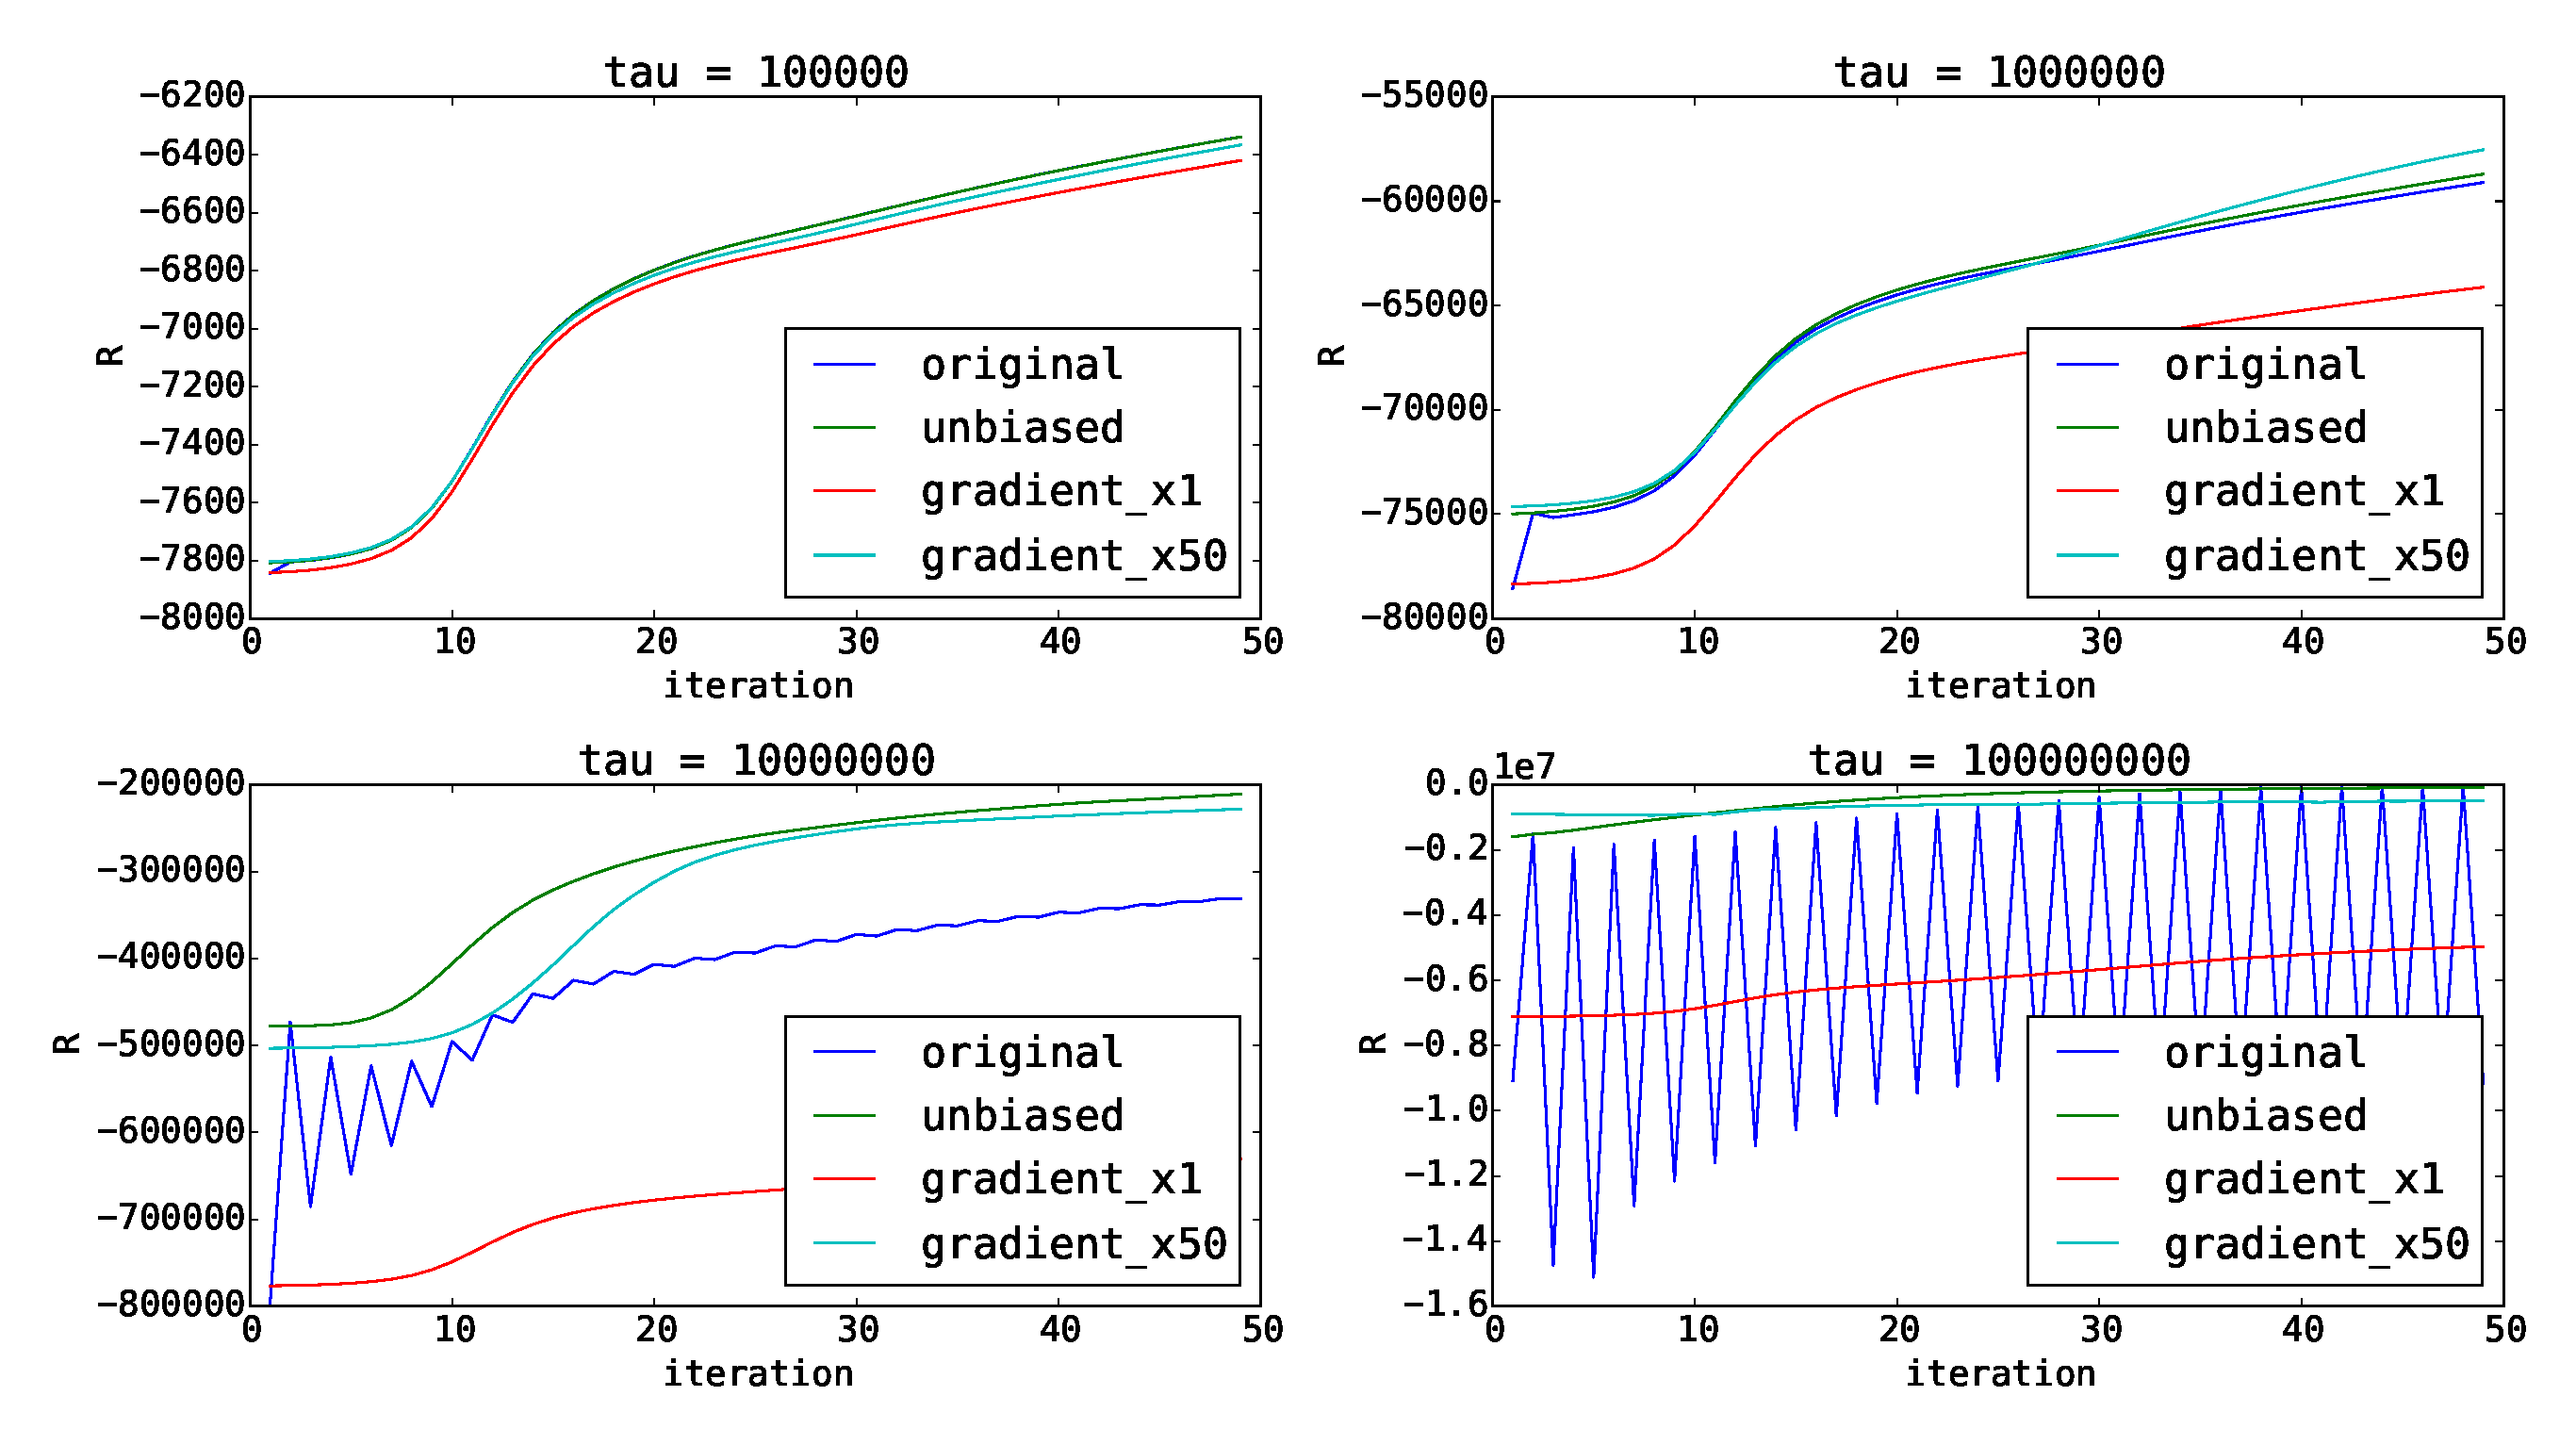
\includegraphics[width=1.0\linewidth]{\hdir//topics_10_R_values}
	\caption{$|T| = 10$. Траектория значений функционала $R$. На верхних графиках виден скачок значений $R$ на первой итераций, на нижних графиках он ярче выражен. Несмещённая модификация и длинный градиент лучше всех остальных.}
\end{figure}

\begin{figure}[!ht]
	\centering  
	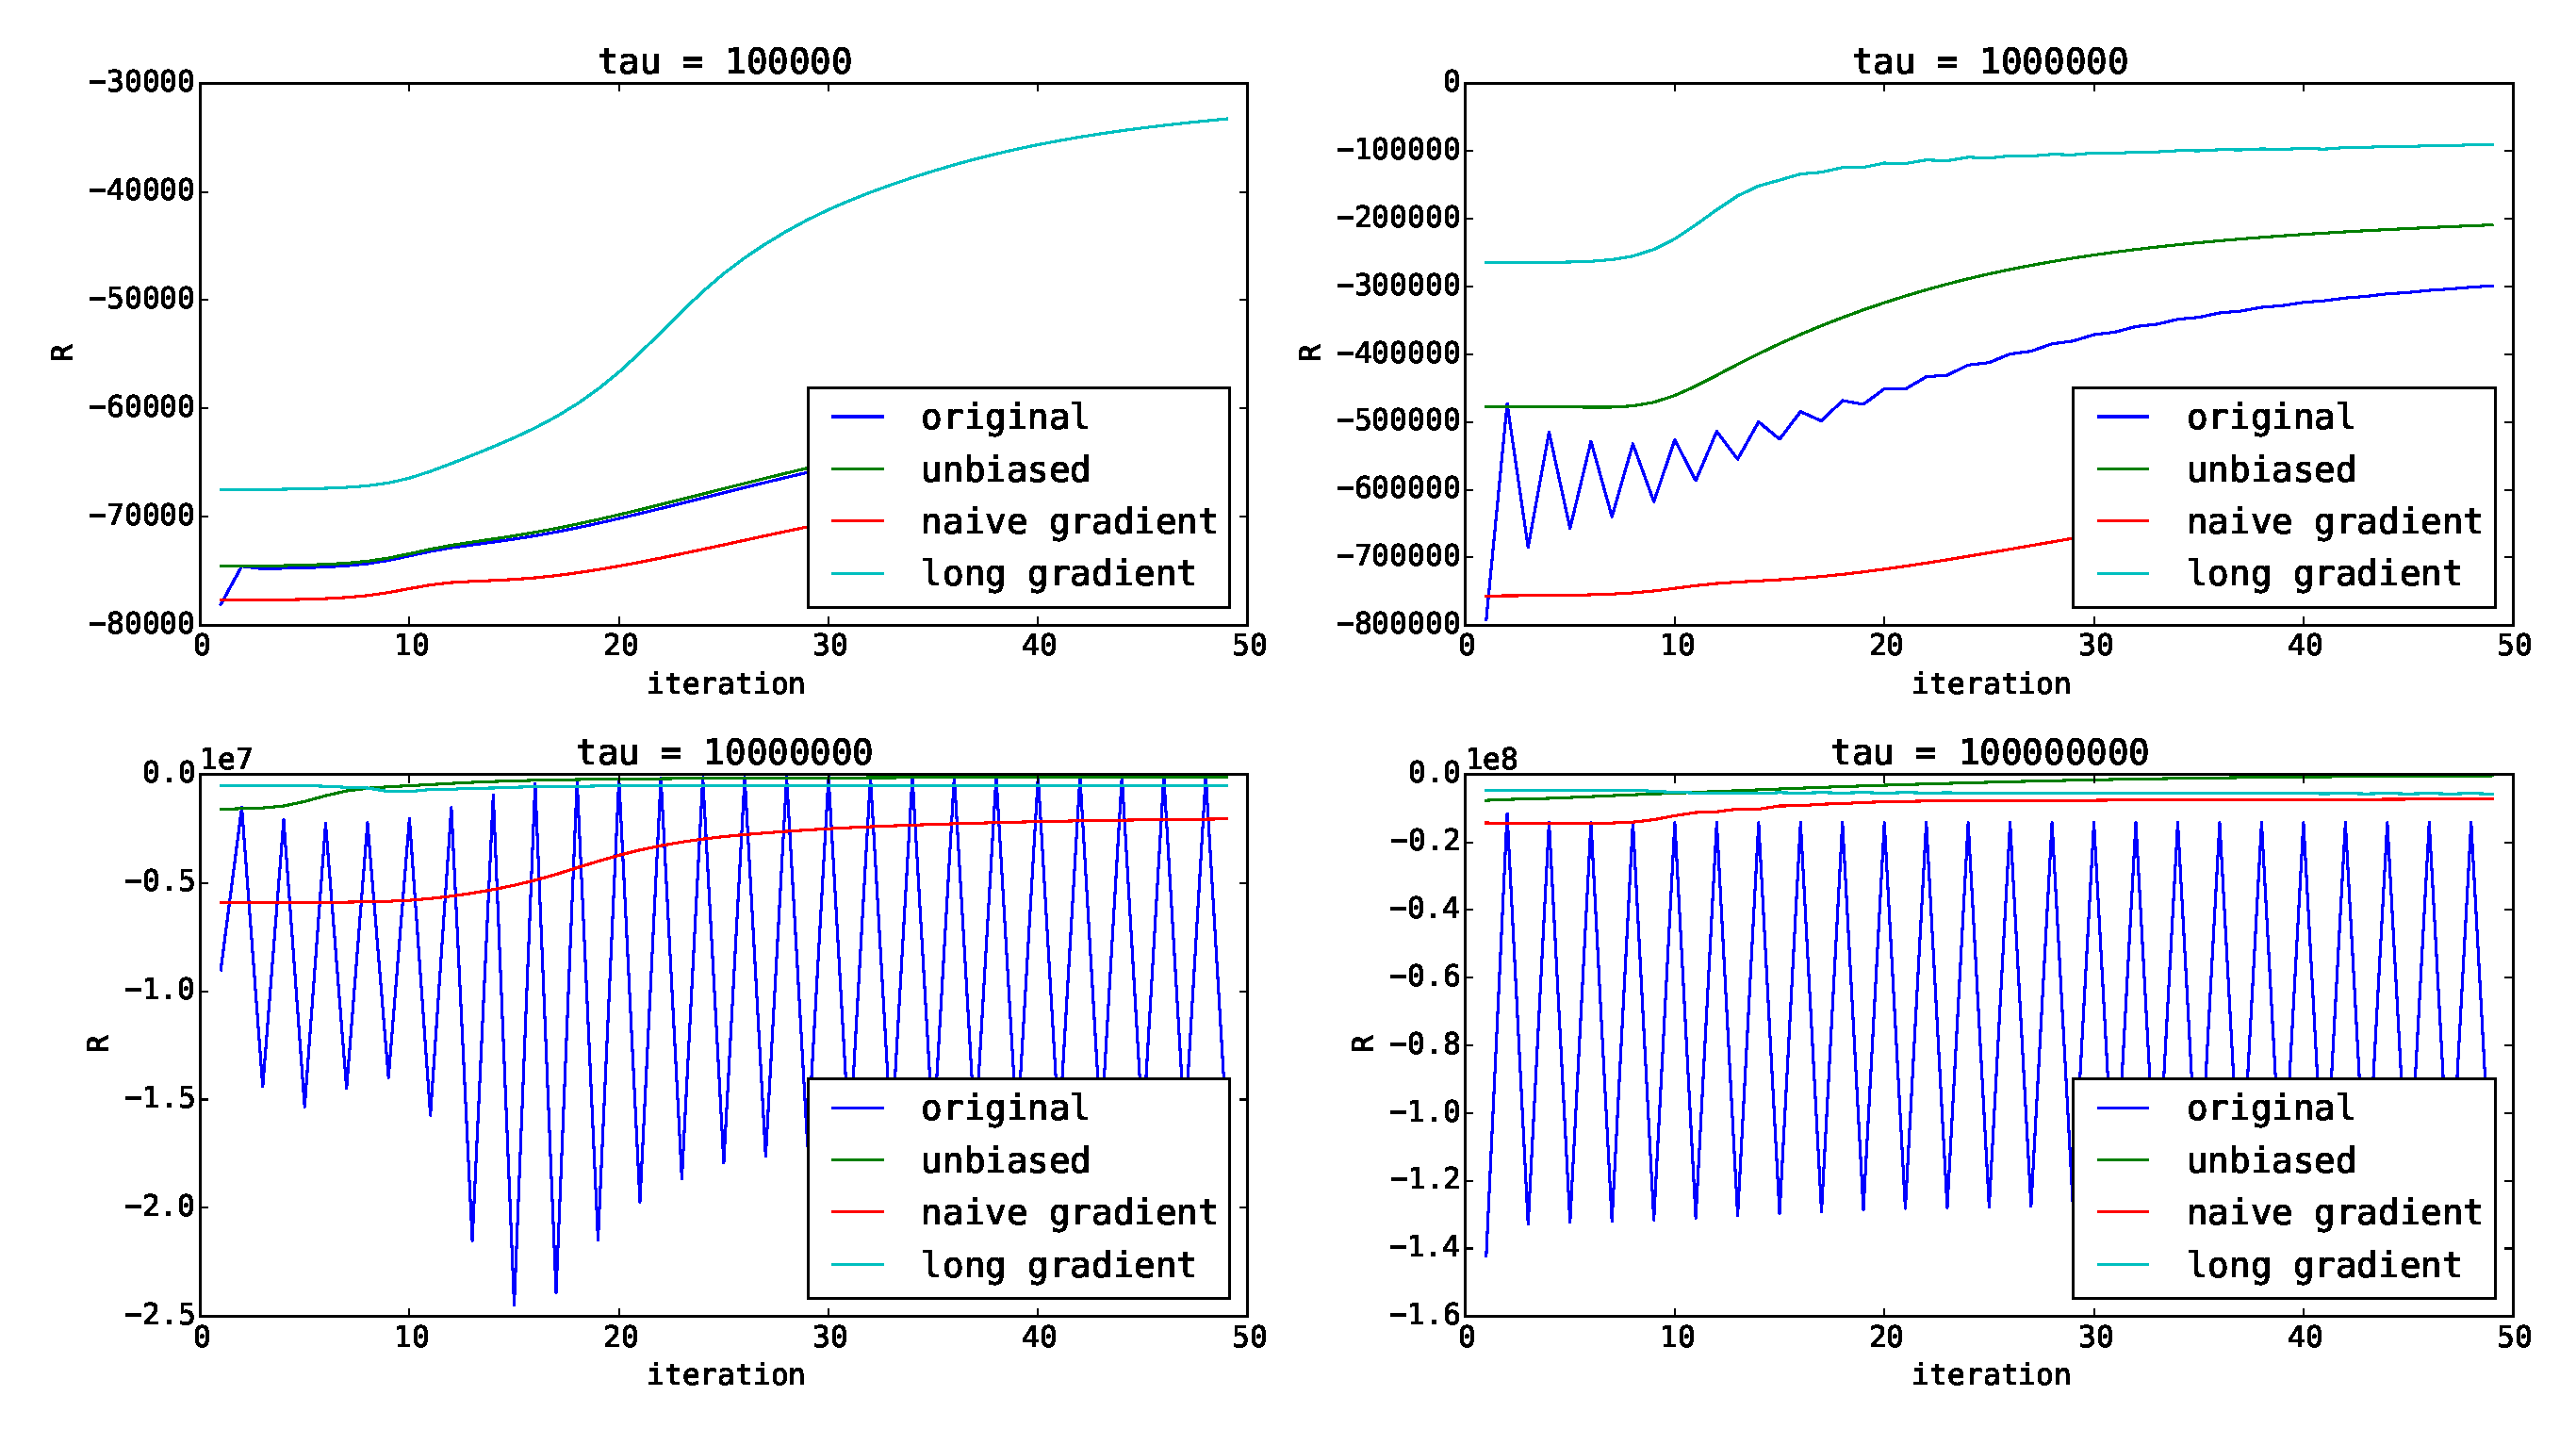
\includegraphics[width=1.0\linewidth]{\hdir//topics_30_R_values}
	\caption{$|T| = 30$. Траектория значений функционала  $R$.  Эффект скачков ярко выражен уже при $\tau = 10^6$. Длинный градиент существенно лучше всех остальных. Наивный градиент существенно отстаёт от других модификаций.}  
\end{figure}

Использование градиента в явном виде заметно хуже остальных. Это связано с тем, что значения $|r_{wt}|$ и $|r_{td}|$ получаются на порядок меньше чем при стандартной формуле или несмещённой модификации, в связи с этим изменение $R$ на М-шаге тоже на порядок меньше. Поэтому использовался градиент, умноженный на 50, чтобы порядок изменения был одинаковый. И эта модификация показала себя при $|T| = 10$ не хуже, а при $|T| = 30$ заметно лучше остальных.

При очень большом значении $\tau$ графики для стандартной и несмещённой оценки резко падают. Этот эффект вызван следующим: стандартные формулы и несмещённая модификация зануляют слишком много параметров, что приводит к падению правдоподобия, поскольку нарушается свойство корректности регуляризатора \ref{fairreg}.

При достаточно больших значения $\tau$ видно, что в стандартной  формуле М-шага есть скачки в изменении $R$ на первых итерациях. Это вызвано тем, что регуляризационные поправки считаются в точке с предыдущей итерации. На первых итерациях  она слабо связана с точкой $\left( \frac{n_{wt}}{{n_t}}, \frac{n_{td}}{n_d}\right)$, к которой применяется регуляризационное преобразование. Конечно, со временем $(\phi_{wt}, \theta_{td})$ стремятся к $\left( \frac{n_{wt}}{{n_t}}, \frac{n_{td}}{n_d}\right)$. Это можно видеть на графиках~--- они постепенно спрямляются. Но на первых итерациях $(\phi_{wt}, \theta_{td})$ существенно отличается  от $\left( \frac{n_{wt}}{{n_t}}, \frac{n_{td}}{n_d}\right)$  и эффект скачков  проявляется, а большое значение $\tau$ усиливает различие и делает эффект более ярким.

С ростом числа тем порядок значений $R$ изменился, и поэтому чувствительность к $\tau$ возросла. Как следствие, можно наблюдать, что колебания значений функционала начинаются раньше, размер этих колебаний существеннее, а градиентные поправки раньше начинают показывать лучшее качество, чем остальные алгоритмы.

\begin{figure}[!ht]
	\centering 
	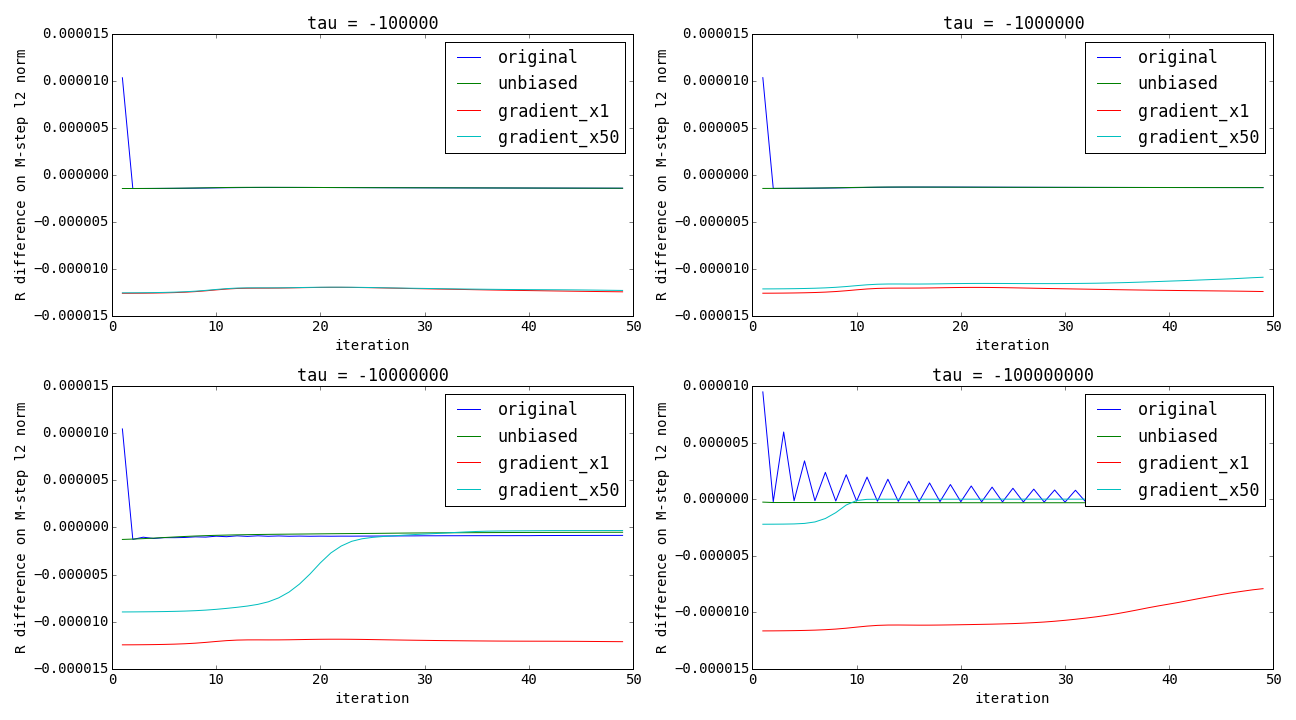
\includegraphics[width=1.0\linewidth]{\hdir//topics_10_RMstepDiffPerL2}
	\caption{$|T| = 10$.  Траектория значений эффективности регуляризационных поправок. Градиентная модификация существенно лучше, однако виден эффект падения для длинного градиента, вызванный приближением к стационарной точке функции $R$. Это означает, что нужно аккуратно подбирать коэффициенты $A_t$ и $B_d$ и, возможно, уменьшать их от итерации к итерации. Эффективность наивного градиента самая высокая поскольку изменение небольшое и работает локальное приближения линейной функцией.}   
\end{figure}

Также была сравнена эффективность регуляризационных поправок. Для этого мы нормировали изменение $R$ на М-шаге на $l_2$ норму этого изменнения. Градиентная модификация на порядок лучше остальных. Это можно объяснить тем, что градиент~--- это оптимальное в $l_2$ направление изменения.

На графиках видно, что при небольших $\tau$ графики для наивного градиента и длинного градиента совпадают, но с ростом $\tau$ они начинают различаться. Это вызвано тем, чтоапрокксимация линейной функцией начинает плохо работать, когда коэффициент перед градиентом слишком большой. Это означает, что этот коэффициент нужно уменьшать с ростом итераций. Это направление для будущего исследования.

Важным свойством при доказательстве сходимости была $\epsilon$-разреживаемость регуляризатора, поэтому требуется проверить выполнение этого условия. На графиках изображены логарифмы минимальных ненулевых значений в матрицах $\Phi$ и $\Theta$.
\begin{figure}[!ht]
	\centering
	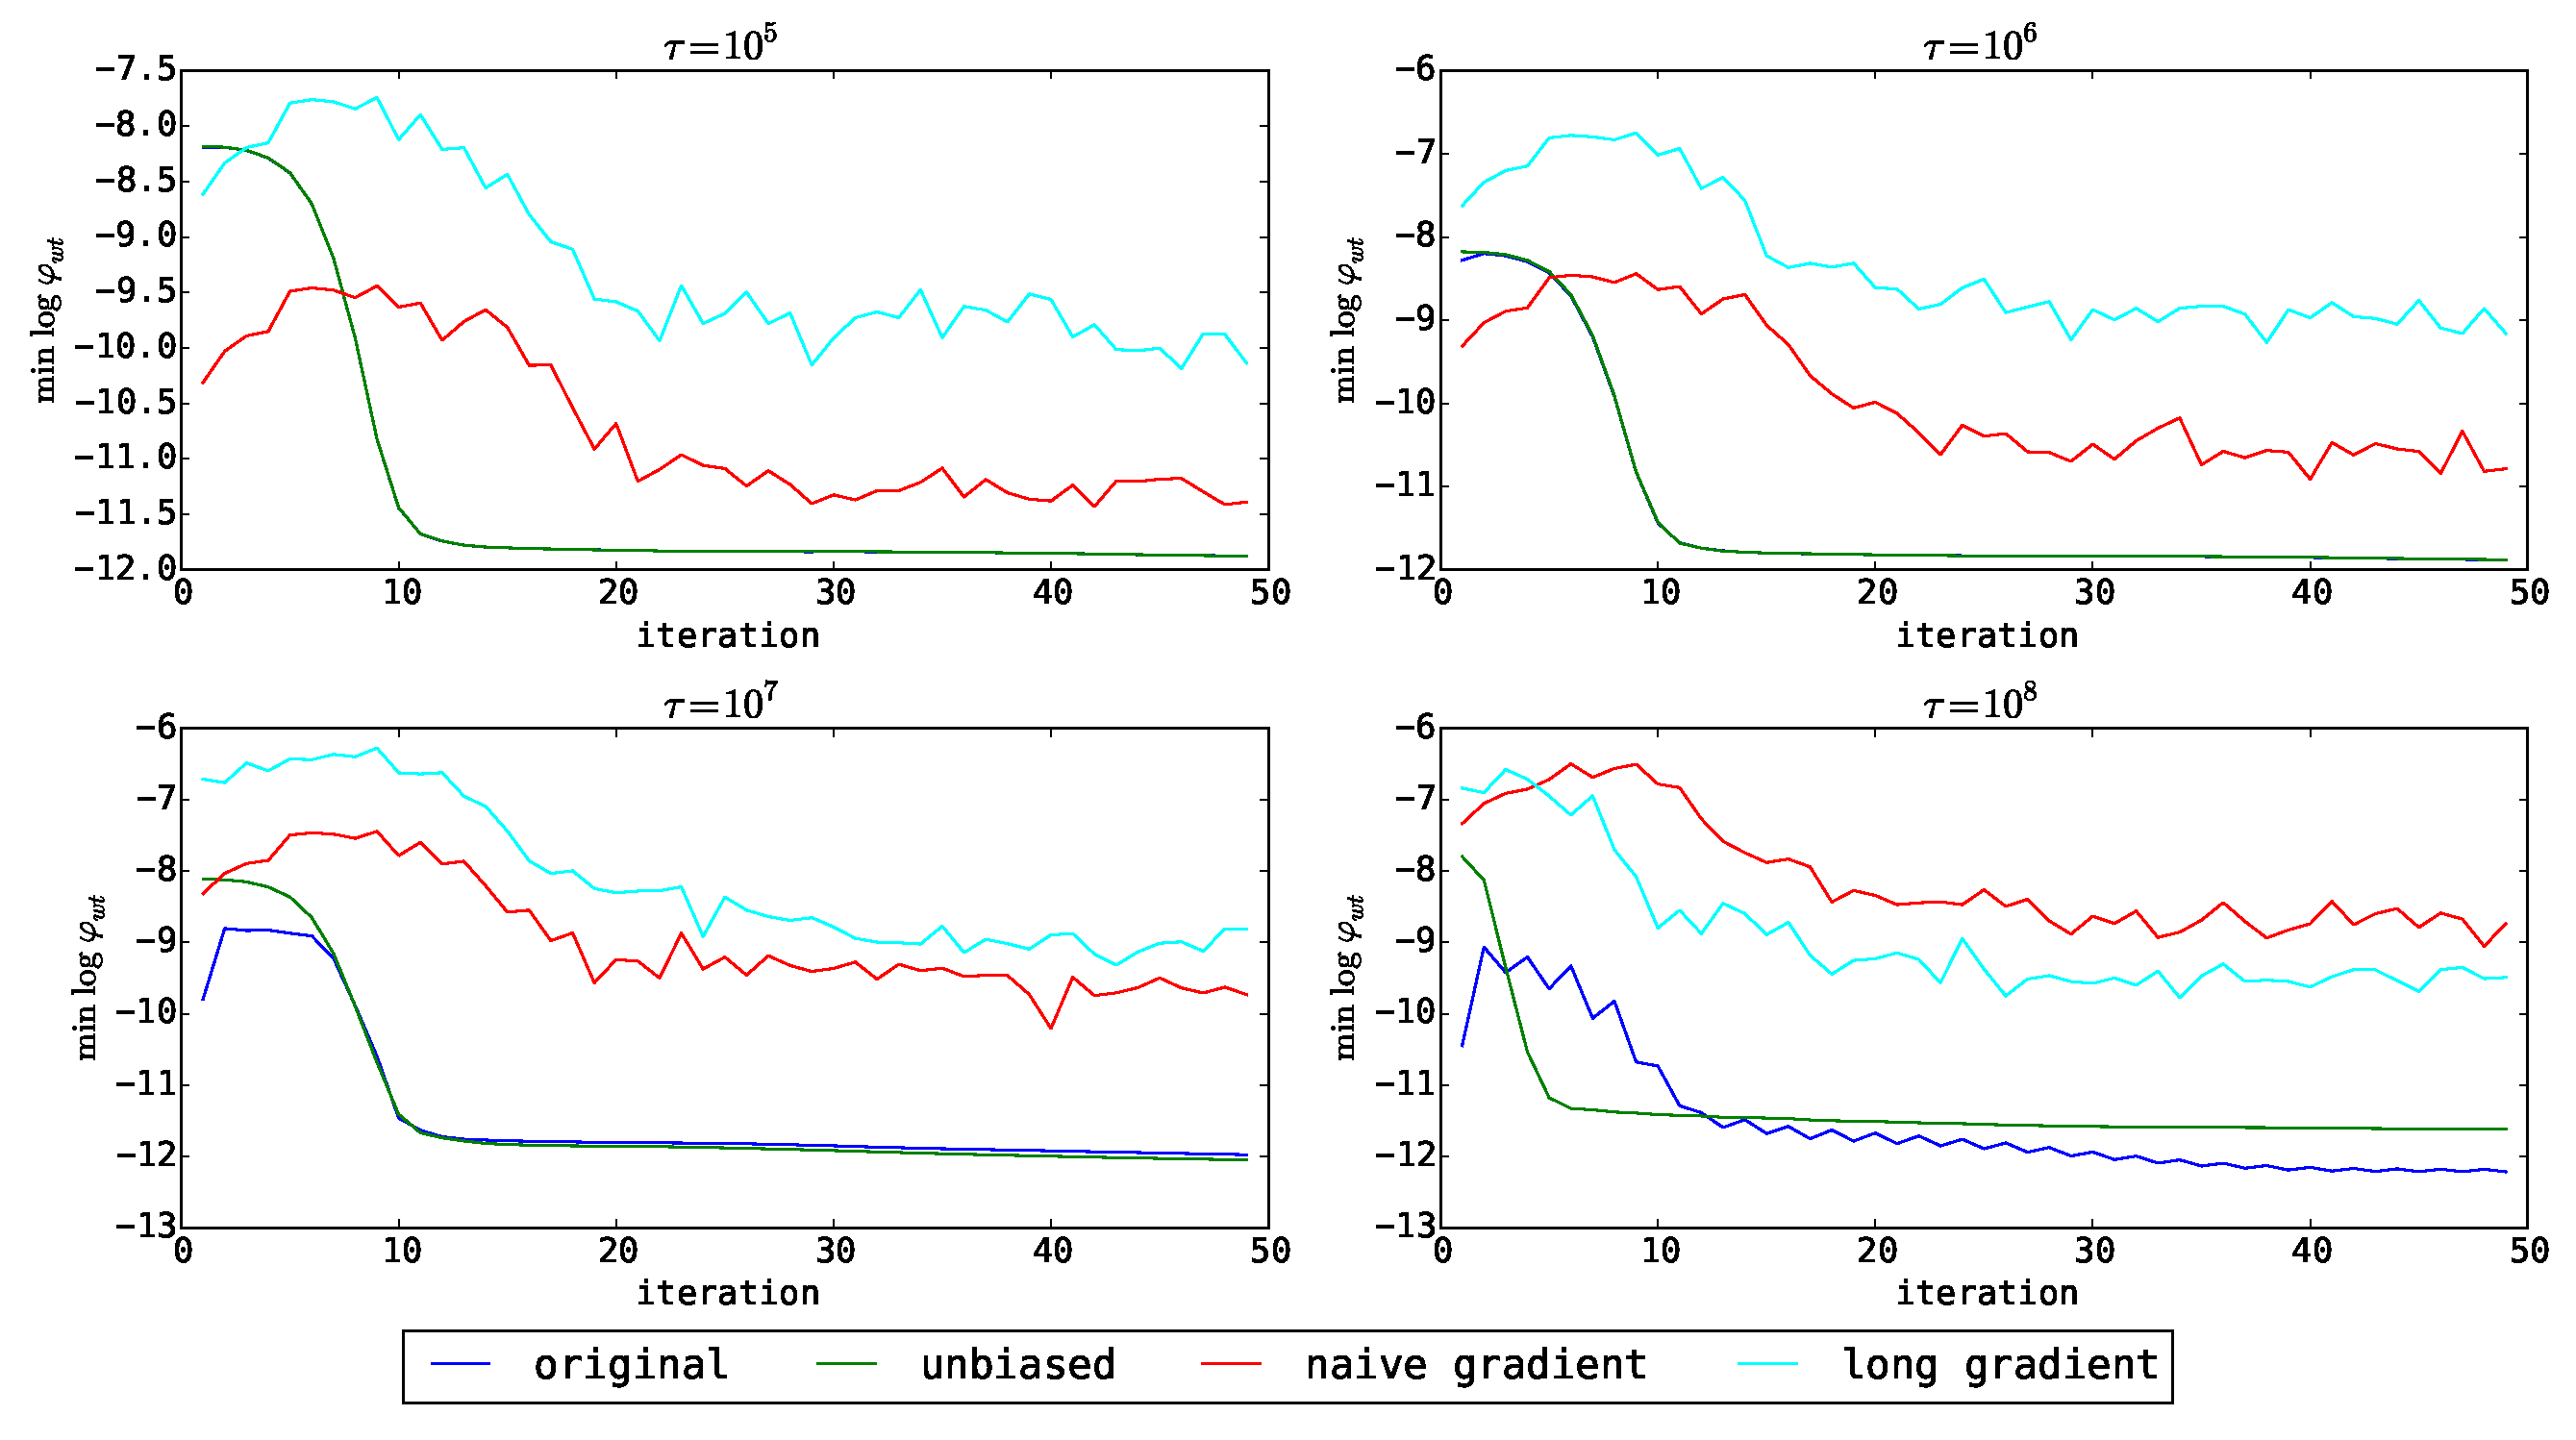
\includegraphics[width=1.0\linewidth]{\hdir//topics_10_minPhi_values}
	\caption{$|T| = 10$. Траектория значений логарифма минимального ненулевого элемента в матрице $\Phi$. Градиентные поправки лучше разреживают матрицу $\Phi$. В матрице $\Theta$ эфеект был одинаковый, так как регуляризатор затрагивает только матрицу $\Phi$.}    
\end{figure}
Несмотря на то, что градиентные методы аккуратнее  зануляют элементы $\Phi$, они делают это заметно лучше -- значения существенно сильнее отделимы от нуля. Однако, в элементах $\Theta$ разницы нет, если не считать случая очень больших $\tau$, когда сильные множественные зануления привели к существенной отделимости параметров от нуля.

Второе важное свойство для сходимости алгоритма~--- это сильная регулярность регуляризатора \ref{strongreg}. Фактически, важна отделимость от нуля знаменателя при нормировке в М-шаге. Именно эти значения  и были получены.

\begin{figure}[!ht]
	\centering  
	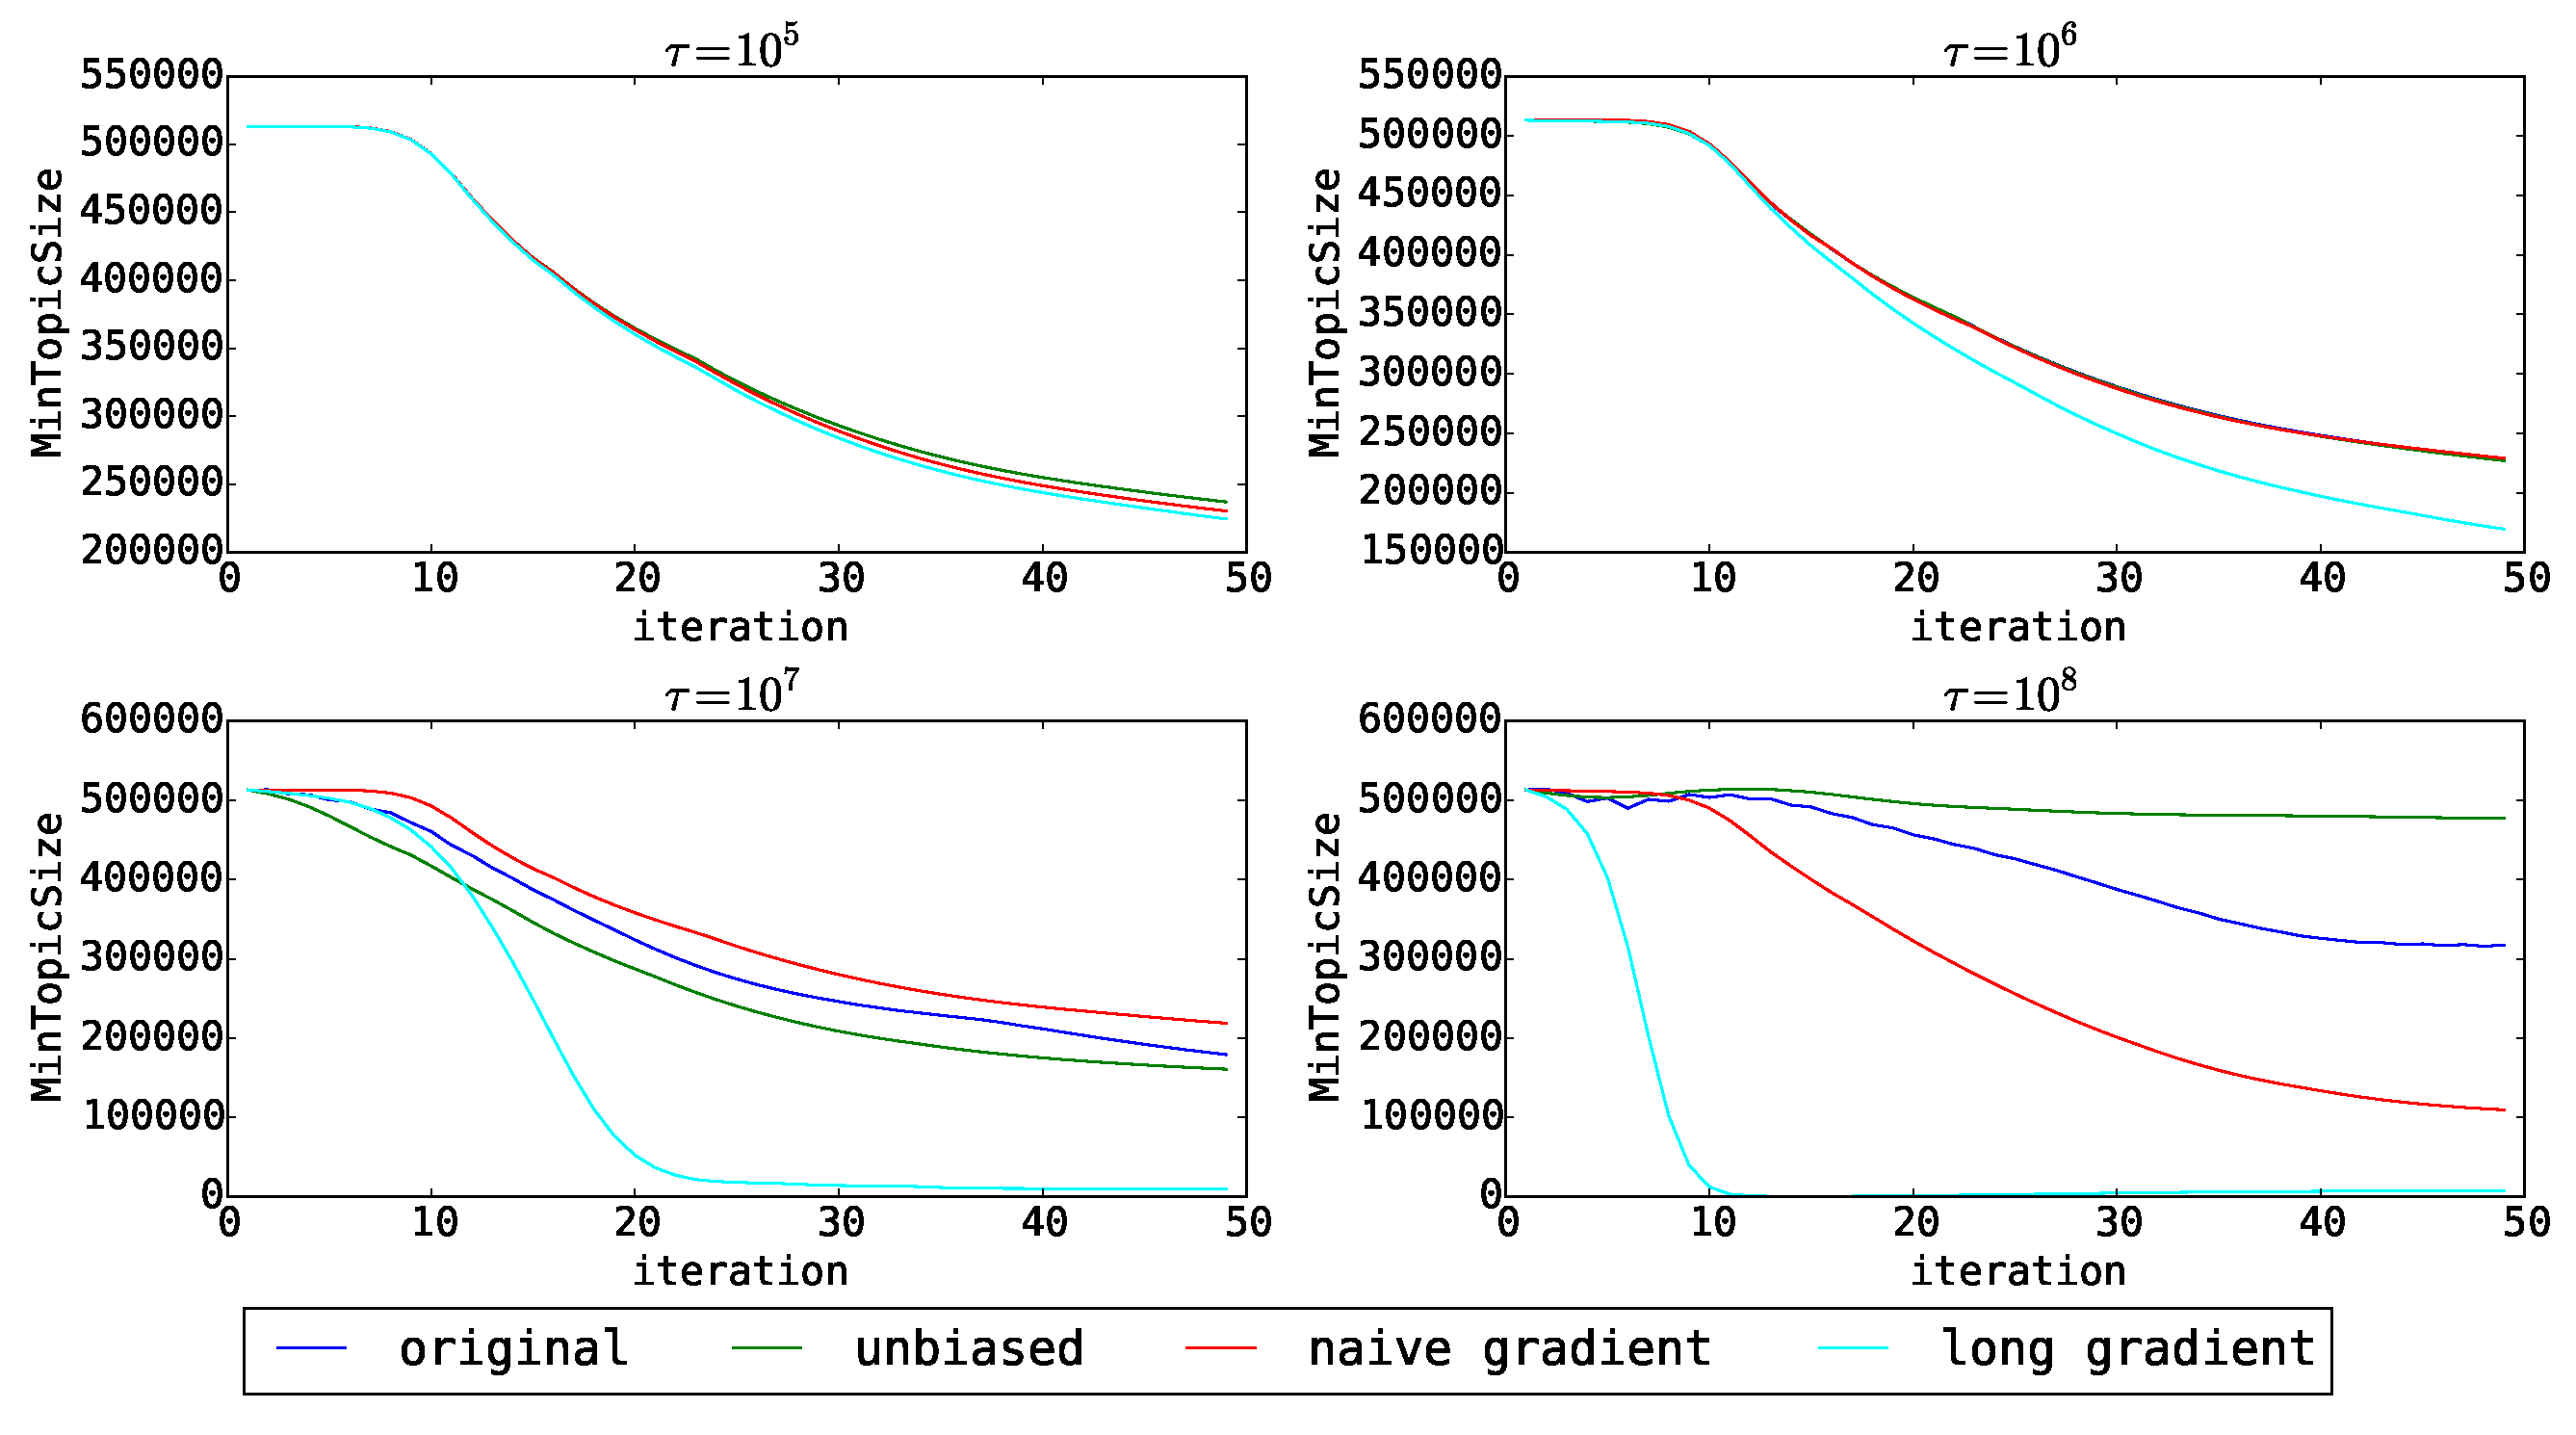
\includegraphics[width=1.0\linewidth]{\hdir//topics_10_MinTopicSize}
	\caption{$|T| = 10$. Траектория значений минимального $n_t$ среди всех тем.}  
\end{figure}

Значения становятся очень малыми, но отделимость от нуля сохраняется (просто отделено небольшой константой порядка 1, но на фоне 10000 это кажется нулём). 

Также видно, что градиентные методы более склонны к селекции тем. Отсюда можно сделать вывод, что градиентное направление обладает большей селективностью, чем стандартная формула. Также стоит отметить, что несмещённая модификация активнее отбирает темы чем стандартная формула.
\paragraph{Итоги экспериментов}
На основании проведённых экспериментов можно сделать следующие выводы:
\begin{enumerate}
\item Предположения о $\epsilon$-отделимости и сильной регулярности выполняются на практике, или могут легко гарантироваться за счёт реализации.
\item С точки зрения оптимизации $L + R$ все рассмотренные формулы отличаются незначительно. Основное достоинтсво предложенных модификаций в этом плане~--- это теоретические гарантии и более эффективная оптимизация $R$ .
\item Есть эффект скачков значений функционалов на первых итерациях для стандартной формулы. Его можно избежать, если пользоваться несмещённой модификацией, для которой есть доказанное утверждение про увеличение $R$, что приводит к более гладкой траектории. Таким образом, модификация явно улучшает стандартную формулу.
\item Для градиентных поправок необходимо дополнительное исследование, чтобы понять как подбирать константу перед градиентом. Эксперименты показали наличие потенциала подобной модификации.
\end{enumerate}
\section{Заключение}
	В вероятностном тематическом моделированиии существует подход ARTM, он предоставляет быстрый и очень гибкий функционал для оптимизации, легко адаптируемый под конкретную задачу. Основная его идея состоит в максимизации регуляризованного правдоподобия при помощи ЕМ алгоритма. На практике предложенный алгоритм успешно сходился, однако, не было теоретического обоснования сходимости. Определение ограничений, при выполнении которых, можно гарантировать сходимость, было целью  работы. Итерации алгоритма ARTM были проинтерпретированы как итерации GEM алгоритма, для которых условия сходимости хорошо изучены. Используя эти результаты, были найдены естественные ограничения на регуляризатор, выполнение которых достаточно просто проверить на практике. Пусть $k$~--- это номер итерации, тогда полученные условия можно сформулировать следующим образом:
\begin{enumerate}
\item Сохранение нуля регуляризатором.
\smallskip

$ n^k_{wt} = 0 \Rightarrow \phi^k_{wt} = 0$ , $n^k_{td} = 0 \Rightarrow \theta^k_{td} = 0$.
\item $\epsilon$-отделимость от нуля элементов матриц $\Phi$ и $\Theta$.
\smallskip

$\exists \epsilon>0\ \exists N\ \forall k > N\ \phi^k_{wt}, \theta^k_{td} \notin (0, \epsilon)$. 
\item  Конечность логарифма правдоподобия на итерациях.
\smallskip

$ n_{dw}>0 \Rightarrow \forall k\ \exists t\colon p^k_{tdw} > 0$.
\item Отделимость от нуля знаменателя на М-шаге.
\smallskip

$\exists \delta >0\ \exists N\ \forall k > N \ \forall t\ \exists w\  n^k_{wt} + r^k_{wt} > \delta$ и аналогичное условие для $\theta$. 
\item Неуменьшение нижней оценки регуляризованного правдоподобия на итерациях.
\smallskip

$\exists N\ \forall k > N\colon\ \ Q^k (\phi^k, \theta^k)+ R(\Phi^k, \Theta^k) \geq Q^k(\phi^{k-1}, \theta^{k-1}) + R(\Phi^{k-1}, \Theta^{k-1})$, где $Q^k(\phi, \Theta) = \sum\limits_{t,d,w} p^k_{tdw} (\ln \phi_{wt} + \ln \theta_{td})$.
\end{enumerate}
Первое условие легко проверяется аналитически. Второе и третье условия можно обеспечить при реализации алгоритма. Четвёртое условие для матрицы $\Phi$ можно проинтерпретировать как критерий селекции тем. То есть, если значение становится меньше $\delta$, то зануляется вся строчка матрицы $\Phi$. С точки зрения реализации это эквивалентно просто удалению строчки в матрице и уменьшению числа тем. Для матрицы $\Theta$ выполнение данного условия можно достичь за счёт выбора $\tau$. Пятое условие должно быть обеспеченно за счёт правильного выбора регуляризационных добавок. Стандартный алгоритм предлагает использовать $r_{wt}^{k} = \phi_{wt}^{k-1} \frac{\partial{R}}{\partial{\phi_{wt}}}(\phi_{wt^{k-1}}, \theta_{td}^{k-1})$ и $r_{td}^{k}=  \theta_{td}^{k-1} \frac{\partial{R}}{\partial{\theta_{td}}}(\phi_{wt}^{k-1}, \theta_{td}^{k-1})$. Для этих формул не удалось получить хороших оценок, поэтому была рассмотрена следующая модификация: замена всех вхождений $\phi_{wt}$ и $\theta_{td}$ на их несмещённые оценки. То есть  $r_{wt}^k=  \frac{n^k_{wt}}{n^k_t}\frac{\partial{R}}{\partial{\phi_{wt}}}\left(\frac{n^k_{wt}}{n^k_t}, \frac{n^k_{td}}{n^k_d}\right)$ и $r_{td}^k=  \frac{n^k_{td}}{n^k_d}\frac{\partial{R}}{\partial{\theta_{td}}}\left(\frac{n^k_{wt}}{n^k_t}, \frac{n^k_{td}}{n^k_d}\right)$. Было предложено рассматривать функцию $R$ не как функцию от $\phi_{wt}$ и $\theta_{td}$, а как функцию от $n_{wt}$ и $n_{td}$, только с нормировкой аргументов. Это позволило получить, что на М-шаге происходит увеличение $R$, если коэффициент регуляризации не слишком велик. Также это подход позволил обобщить ARTM на случай, когда регуляризатор зависит не только от $\Phi$  и $\Theta$ но и от параметров М-шага. Вычисленный градиент $R$ использовался  в качестве регуляризационных добавок на М-шаге: $r^k_{wt} =  A_t \bigl[{\frac{\partial{R}}{\partial{\phi_{wt}}} - \sum\limits_u \phi_{ut} \frac{\partial{R}}{\partial{\phi_{ut}}} }\bigr] \left(\frac{n^k_{wt}}{n^k_t}, \frac{n^k_{td}}{n^k_d}\right)$ и $r^k_{td} =  B_d \bigl[ {\frac{\partial{R}}{\partial{\theta_{td}}} - \sum\limits_s \theta_{sd} \frac{\partial{R}}{\partial{\theta_{sd}}} }\bigr] \left(\frac{n^k_{wt}}{n^k_t}, \frac{n^k_{td}}{n^k_d}\right)$.

Был проведён эксперимент, в котором сравнивались три возможных формулы М-шага. Предложенные модификации показали улучшение по сравнению со стандартными формулами. Для будущего исследования выделен вопрос управления коэффициентом перед градиентом регуляризатора в градиентной модификации М-шага.

\begin{thebibliography}{10}
\def\selectlanguageifdefined#1{
\expandafter\ifx\csname date#1\endcsname\relax
\else\selectlanguage{#1}\fi}

\bibitem{hofmann1999probabilistic}
\selectlanguageifdefined{english}
\emph{Hofmann~T.}
Probabilistic latent semantic indexing~//
Proceedings of the 22nd annual international ACM SIGIR conference on Research
  and development in information retrieval.~---
1999.
P.~50--57.

\bibitem{daud2010knowledge}
\selectlanguageifdefined{english}
\emph{Daud~A., Li~J., Zhou~L., Muhammad~F.}
Knowledge discovery through directed probabilistic topic models: a survey~//
Frontiers of computer science in China,
2010.
Vol.~4.
No.~2.
P.~280--301.
doi:~\url{http://dx.doi.org/10.1007/s11704-009-0062-y}.

\bibitem{blei2003latent}
\selectlanguageifdefined{english}
\emph{Blei~D.~M., Ng~A.~Y., Jordan~M.~I.}
Latent dirichlet allocation~//
the Journal of machine Learning research,
2003.
Vol.~3.
P.~993--1022.

\bibitem{cohn2001missing}
\selectlanguageifdefined{english}
\emph{Cohn~D., Hofmann~T.}
The missing link-a probabilistic model of document content and hypertext
  connectivity~//
Advances in neural information processing systems,
2001.
P.~430--436.

\bibitem{mccallum2005author}
\selectlanguageifdefined{english}
\emph{McCallum~A., Corrada-Emmanuel~A., Wang~X.}
The author-recipient-topic model for topic and role discovery in social
  networks: Experiments with enron and academic email,
2005.

\bibitem{nallapati2008link}
\selectlanguageifdefined{english}
\emph{Nallapati~R., Cohen~W.~W.}
Link-plsa-lda: A new unsupervised model for topics and influence of blogs~//
ICWSM.~---
2008.

\bibitem{steyvers2004probabilistic}
\selectlanguageifdefined{english}
\emph{Steyvers~M., Smyth~P., Rosen-Zvi~M., Griffiths~T.}
Probabilistic author-topic models for information discovery~//
Proceedings of the tenth ACM SIGKDD international conference on Knowledge
  discovery and data mining.~---
2004.
P.~306--315.

\bibitem{gruber2007hidden}
\selectlanguageifdefined{english}
\emph{Gruber~A., Weiss~Y., Rosen-Zvi~M.}
Hidden topic markov models~//
International conference on artificial intelligence and statistics.~---
2007.
P.~163--170.

\bibitem{wallach2006topic}
\selectlanguageifdefined{english}
\emph{Wallach~H.~M.}
Topic modeling: beyond bag-of-words~//
Proceedings of the 23rd international conference on Machine learning.~---
2006.
P.~977--984.

\bibitem{bilmes1998gentle}
\selectlanguageifdefined{english}
\emph{Bilmes~J.~A. et~al.}
A gentle tutorial of the em algorithm and its application to parameter
  estimation for gaussian mixture and hidden markov models~//
International Computer Science Institute,
1998.
Vol.~4.
No. 510.
P.~126.

\bibitem{jordan1999introduction}
\selectlanguageifdefined{english}
\emph{Jordan~M.~I., Ghahramani~Z., Jaakkola~T.~S., Saul~L.~K.}
An introduction to variational methods for graphical models~//
Machine learning,
1999.
Vol.~37.
No.~2.
P.~183--233.
doi:~\url{http://dx.doi.org/10.1007/978-94-011-5014-9_5}.

\bibitem{gilks1996introducing}
\selectlanguageifdefined{english}
\emph{Gilks~W.~R., Richardson~S., Spiegelhalter~D.~J.}
Introducing markov chain monte carlo~//
Markov chain Monte Carlo in practice,
1996.
Vol.~1.
P.~19.

\bibitem{andrieu2003introduction}
\selectlanguageifdefined{english}
\emph{Andrieu~C., De~Freitas~N., Doucet~A., Jordan~M.~I.}
An introduction to mcmc for machine learning~//
Machine learning,
2003.
Vol.~50.
No. 1-2.
P.~5--43.

\bibitem{griffiths2004finding}
\selectlanguageifdefined{english}
\emph{Griffiths~T.~L., Steyvers~M.}
Finding scientific topics~//
Proceedings of the National Academy of Sciences,
2004.
Vol. 101.
No. suppl 1.
P.~5228--5235.
doi:~\url{http://dx.doi.org/10.1073/pnas.0307752101}.

\bibitem{vorontsov2014additive}
\selectlanguageifdefined{english}
\emph{Vorontsov~K.}
Additive regularization for topic models of text collections~//
Doklady Mathematics.~---
2014.
Vol.~89.
P.~301--304.

\bibitem{vorontsov2014tutorial}
\selectlanguageifdefined{english}
\emph{Vorontsov~K., Potapenko~A.}
Tutorial on probabilistic topic modeling: additive regularization for
  stochastic matrix factorization~//
Analysis of Images, Social networks and Texts.~---
2014.
P.~29--46.

\bibitem{vorontsov2015additive}
\selectlanguageifdefined{english}
\emph{Vorontsov~K., Potapenko~A.}
Additive regularization of topic models~//
Machine Learning,
2015.
Vol. 101.
No. 1-3.
P.~303--323.
doi:~\url{http://dx.doi.org/10.1007/s10994-014-5476-6}.

\bibitem{dempster1977maximum}
\selectlanguageifdefined{english}
\emph{Dempster~A.~P., Laird~N.~M., Rubin~D.~B.}
Maximum likelihood from incomplete data via the em algorithm~//
Journal of the royal statistical society. Series B (methodological),
1977.
P.~1--38.

\bibitem{wu1983convergence}
\selectlanguageifdefined{english}
\emph{Wu~C.~J.}
On the convergence properties of the em algorithm~//
The Annals of statistics,
1983.
P.~95--103.
doi:~\url{http://dx.doi.org/10.1214/aos/1176346060}.

\bibitem{topsoe2000some}
\selectlanguageifdefined{english}
\emph{Tops{\o}e~F.}
Some inequalities for information divergence and related measures of
  discrimination~//
Information Theory, IEEE Transactions on,
2000.
Vol.~46.
No.~4.
P.~1602--1609.
doi:~\url{http://dx.doi.org/10.1109/18.850703}.

\end{thebibliography}


\maketitleSecondary
\English

\begin{thebibliography}{10}
\def\selectlanguageifdefined#1{
\expandafter\ifx\csname date#1\endcsname\relax
\else\selectlanguage{#1}\fi}

\bibitem{hofmann1999probabilistic}
\selectlanguageifdefined{english}
Hofmann, T.
1999.
Probabilistic latent semantic indexing.
\emph{Proceedings of the 22nd annual international ACM SIGIR conference on
  Research and development in information retrieval}.
50--57.

\bibitem{daud2010knowledge}
\selectlanguageifdefined{english}
Daud, A., J.~Li, L.~Zhou,  and F.~Muhammad.
2010.
Knowledge discovery through directed probabilistic topic models: a survey.
\emph{Frontiers of computer science in China}
4(2):280--301.
doi:~\url{http://dx.doi.org/10.1007/s11704-009-0062-y}.

\bibitem{blei2003latent}
\selectlanguageifdefined{english}
Blei, D.~M., A.~Y. Ng,  and M.~I. Jordan.
2003.
Latent dirichlet allocation.
\emph{the Journal of machine Learning research}
3:993--1022.

\bibitem{cohn2001missing}
\selectlanguageifdefined{english}
Cohn, D.,  and T.~Hofmann.
2001.
The missing link-a probabilistic model of document content and hypertext
  connectivity.
\emph{Advances in neural information processing systems}
430--436.

\bibitem{mccallum2005author}
\selectlanguageifdefined{english}
McCallum, A., A.~Corrada-Emmanuel,  and X.~Wang.
2005.
The author-recipient-topic model for topic and role discovery in social
  networks: Experiments with enron and academic email .

\bibitem{nallapati2008link}
\selectlanguageifdefined{english}
Nallapati, R.,  and W.~W. Cohen.
2008.
Link-plsa-lda: A new unsupervised model for topics and influence of blogs.
\emph{ICWSM}.

\bibitem{steyvers2004probabilistic}
\selectlanguageifdefined{english}
Steyvers, M., P.~Smyth, M.~Rosen-Zvi,  and T.~Griffiths.
2004.
Probabilistic author-topic models for information discovery.
\emph{Proceedings of the tenth ACM SIGKDD international conference on Knowledge
  discovery and data mining}.
306--315.

\bibitem{gruber2007hidden}
\selectlanguageifdefined{english}
Gruber, A., Y.~Weiss,  and M.~Rosen-Zvi.
2007.
Hidden topic markov models.
\emph{International conference on artificial intelligence and statistics}.
163--170.

\bibitem{wallach2006topic}
\selectlanguageifdefined{english}
Wallach, H.~M.
2006.
Topic modeling: beyond bag-of-words.
\emph{Proceedings of the 23rd international conference on Machine learning}.
977--984.

\bibitem{bilmes1998gentle}
\selectlanguageifdefined{english}
Bilmes, J.~A. et~al.
1998.
A gentle tutorial of the em algorithm and its application to parameter
  estimation for gaussian mixture and hidden markov models.
\emph{International Computer Science Institute}
4(510):~126.

\bibitem{jordan1999introduction}
\selectlanguageifdefined{english}
Jordan, M.~I., Z.~Ghahramani, T.~S. Jaakkola,  and L.~K. Saul.
1999.
An introduction to variational methods for graphical models.
\emph{Machine learning}
37(2):183--233.
doi:~\url{http://dx.doi.org/10.1007/978-94-011-5014-9_5}.

\bibitem{gilks1996introducing}
\selectlanguageifdefined{english}
Gilks, W.~R., S.~Richardson,  and D.~J. Spiegelhalter.
1996.
Introducing markov chain monte carlo.
\emph{Markov chain Monte Carlo in practice}
1:~19.

\bibitem{andrieu2003introduction}
\selectlanguageifdefined{english}
Andrieu, C., N.~De~Freitas, A.~Doucet,  and M.~I. Jordan.
2003.
An introduction to mcmc for machine learning.
\emph{Machine learning}
50(1-2):5--43.

\bibitem{griffiths2004finding}
\selectlanguageifdefined{english}
Griffiths, T.~L.,  and M.~Steyvers.
2004.
Finding scientific topics.
\emph{Proceedings of the National Academy of Sciences}
101(suppl 1):5228--5235.
doi:~\url{http://dx.doi.org/10.1073/pnas.0307752101}.

\bibitem{vorontsov2014additive}
\selectlanguageifdefined{english}
Vorontsov, K.
2014.
Additive regularization for topic models of text collections.
\emph{Doklady Mathematics}.
89(3):301--304.

\bibitem{vorontsov2014tutorial}
\selectlanguageifdefined{english}
Vorontsov, K.,  and A.~Potapenko.
2014.
Tutorial on probabilistic topic modeling: additive regularization for
  stochastic matrix factorization.
\emph{Analysis of Images, Social networks and Texts}.
Springer.
29--46.

\bibitem{vorontsov2015additive}
\selectlanguageifdefined{english}
Vorontsov, K.,  and A.~Potapenko.
2015.
Additive regularization of topic models.
\emph{Machine Learning}
101(1-3):303--323.
doi:~\url{http://dx.doi.org/10.1007/s10994-014-5476-6}.

\bibitem{dempster1977maximum}
\selectlanguageifdefined{english}
Dempster, A.~P., N.~M. Laird,  and D.~B. Rubin.
1977.
Maximum likelihood from incomplete data via the em algorithm.
\emph{Journal of the royal statistical society. Series B (methodological)}
1--38.

\bibitem{wu1983convergence}
\selectlanguageifdefined{english}
Wu, C.~J.
1983.
On the convergence properties of the em algorithm.
\emph{The Annals of statistics}
95--103.
doi:~\url{http://dx.doi.org/10.1214/aos/1176346060}.

\bibitem{topsoe2000some}
\selectlanguageifdefined{english}
Tops{\o}e, F.
2000.
Some inequalities for information divergence and related measures of
  discrimination.
\emph{Information Theory, IEEE Transactions on}
46(4):1602--1609.
doi:~\url{http://dx.doi.org/10.1109/18.850703}.

\end{thebibliography}


\end{document}
